\chapter{Grundlagen der Schmerzbewertung mit Hilfe akustischer Signale}
\label{sec:foundations}

%Nochemal lesen!
Das Ziel dieses Kapitels ist es, wichtige Grundlagen zu erläutern, die zum Verständnis des in dieser Arbeit vorgestellten Konzeptes und den dabei angewandten Methoden notwendig sind. Dazu werden in \autoref{sec:signal_foundations} zunächst einige Teilaspekte der Audiosignalverarbeitung besprochen, welche insbesondere bei der akustischen Modellierung der menschlichen Stimme Anwendung finden. In \autoref{sec:medicalFoundations} werden Methoden zur Schmerzbewertung bei Neugeborenen beschrieben. Die Schmerzdiagnostik wird zunächst aus Sicht medizinischer Fachkräfte im klinischen Alltag beleuchtet. Weiterhin wird eine Einführung in die \glqq Schreiforschung\grqq{} gegeben, einem Wissenschaftsgebiet, bei dem das Weinen von Neugeborenen mit Methoden der Signalverarbeitung tiefergehend analysiert wird. In \autoref{sec:learning} werden Grundlagen des überwachten maschinellen Lernens erläutert, da diese im Zusammenhang mit der Erkennung von Schreigeräuschen in Audiosignalen sowie der automatisierten Schmerzbewertung Einsatz finden.

\section{Grundlagen der Verarbeitung akustischer Signale}
\label{sec:signal_foundations}

Der erste Schritt zur Schmerzdiagnostik auf Basis akustischer Informationen des Weinens von Neugeborenen ist, dieses Weinen mit einem Mikrofon aufzunehmen und in ein digitales Signal zu wandeln. In diesem Abschnitt werden Grundlagen zur Verarbeitung eines solchen digitalen Signals erläutert. Es wird ein grundlegendes Verständnis dieses Bereichs vorausgesetzt. Falls dieses Verständnis nicht vorhanden ist, wird zur Einarbeitung das Buch \glqq The Scientist and Engineer's Guide to Digital Signal Processing\grqq{} von Steven W. Smith empfohlen \cite{dspGuide}, welches vom Autor kostenlos als E-Book bereitgestellt wird.

\subsection{Grundlegende Definitionen}

Ein digitales Signal $x[\;]$ ist eine beliebige Zahlenfolge mit diskretem Definitionsbereich. Dem Definitionsbereich kommt die Bedeutung \emph{Zeit} zu.\cite[S. 11-12]{dspGuide} In dieser Arbeit gilt die Konvention, dass mit $x[\;]$ das \emph{gesamte} Signal und mit $x[n]$ \emph{ein} Wert des Signals zum \emph{Zeitpunkt} oder \emph{Index} $n$ gemeint ist. Ein Wert $x[n]$ wird auch als \emph{Sample} bezeichnet. Die Samplingfrequenz des digitalen Signals wird mit $f_s$ bezeichnet.

Der Indexbereich eines Signals erstreckt sich implizit immer von negativer bis positiver Unendlichkeit. Das heißt nicht, dass alle Samples des Signals auch Informationen enthalten müssen. Der \emph{Support} ist das kleinst mögliche Zeitintervall, außerhalb dessen alle Samples des Signals den Wert 0 haben, wie \autoref{eq:support} definiert. Ein Sample mit dem Wert 0 wird in dieser Arbeit auch als \glqq 0-Sample\grqq{} bezeichnet.\cite[S. 24]{dspMichigan}

\begin{equation}
\label{eq:support}
\begin{split}
\text{Sup}(x[\;]) = [sup_s, sup_e] \quad , sup_s, sup_e \in \mathbb{Z} \\  \forall n \not\in [sup_s, sup_e] : x[n] = 0
\end{split}
\end{equation}

Die \emph{Dauer} eines Signals entspricht der Länge des Supportes nach \autoref{eq:duration}. In dieser Arbeit gilt die Konvention, dass die Länge eines Signals mit der Variable $N$ abgekürzt wird. Wenn nicht explizit anders definiert, erstreckt sich der Support eines Signals über das Intervall $0 ,\ldots, N-1$.\cite[S. 24]{dspMichigan}

\begin{equation}
\text{Length}(x[\;]) = sup_e - sup_s + 1 = N
\label{eq:duration}
\end{equation}


\subsection{Statistische Merkmale von Signalen}

Im folgenden wird ein Überblick über wichtige statistische Merkmale von Signalen gegeben.

\begin{enumerate}[leftmargin=*]
	
	\item Der \textbf{Maximalwert/Minimalwert} beschreibt den höchsten/niedrigsten in  $x[\;]$ enthaltenen Wert nach \autoref{eq:maxAndMin}.
	
	\begin{equation}
	\begin{gathered}
	\max(x[\;]) = \max\limits_{n \in \text{Sup}(x[\;]) }\{\ x[n]\ \} \\ 
	\min(x[\;])= \min\limits_{n \in \text{Sup}(x[\;])}\{\ x[n]\ \}
	\end{gathered}
	\label{eq:maxAndMin}
	\end{equation}
	
	
	\item Der \textbf{Durchschnittswert} (engl. \emph{Average Value}) beschreibt den durchschnittlichen Wert aller Samples von $x[\;]$ nach \autoref{eq:avg}.
	
	\begin{equation}
	\text{AVG}(x[\;]) = \frac{1}{N} \sum_{n = 0}^{N-1} x[n]
	\label{eq:avg}
	\end{equation}
	
	\item Der \textbf{Mean Squared Value} (\emph{MSV}) beschreibt den Durchschnittswert aller quadrierten Samples nach \autoref{eq:msv}. Er wird auch als \emph{durchschnittliche Energie} oder \emph{average Power} bezeichnet.
	
	\begin{equation}
	\text{MSV}(x[\;]) = \frac{1}{N} \sum_{n = 0}^{N-1} x[n]^2
	\label{eq:msv}
	\end{equation}
	
	\item Der \textbf{Root Mean Square} (\emph{RMS}) wird definiert als die Wurzel des Mean Squared Value nach \autoref{eq:rms}. Der RMS kann im Vergleich zum MSV intuitiver ins Verhältnis zu den Werten des Signals gesetzt werden kann. Er wird im Deutschen auch als \textbf{Effektivwert} oder \textbf{Durchschnittsleistung} bezeichnet.
	
	\begin{equation}
	\text{RMS}(x[\;]) = \sqrt{\frac{1}{N} \sum_{n = 0}^{N-1} x[n]^2}
	\label{eq:rms}
	\end{equation}
	
	\item Die \textbf{Energie} (engl. \emph{Energy}) eines Signals wird nach \autoref{eq:energy} definiert. Sie entspricht dem MSV-Wert multipliziert mit der Länge des Intervalls.\cite[S. 27-28]{dspMichigan}
	
	\begin{equation}
	\text{E}(x[\;]) = \sum_{n = 0}^{N-1} x[n]^2
	\label{eq:energy}
	\end{equation}
	
\end{enumerate}	

%\begin{figure}[h]
%	\centering
%	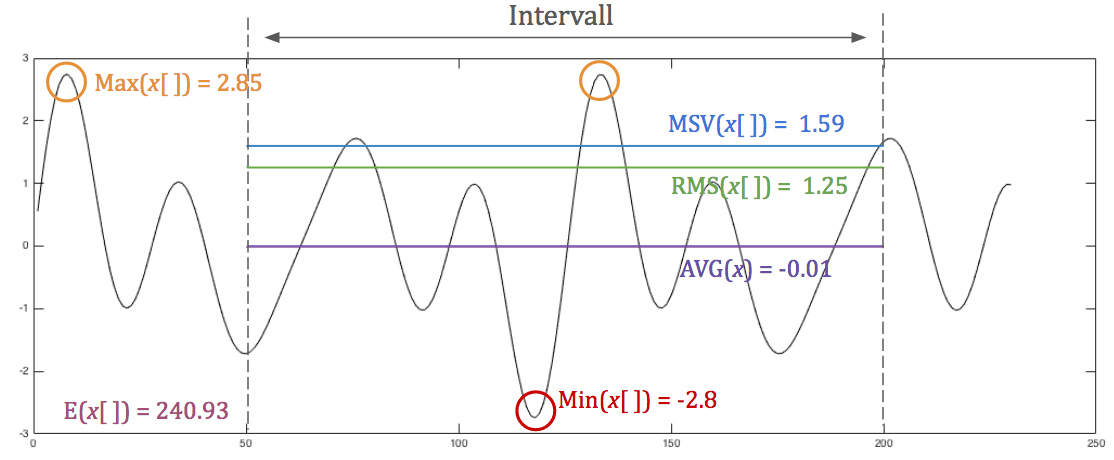
\includegraphics[width=0.9\textwidth]{bilder/sigStats02.png}
%	\caption{Statistische Merkmale eines Beispielsignals über dem Intervall [50,200]}
%	\label{img:sigStats}
%\end{figure}

\subsection{Fehlersignale}

Angenommen, ein Signal $x[\;]$ wird übertragen, auf dem Übertragungsweg jedoch durch ein anderes Störsignal, wie z.B. Rauschen, $e[\;]$ überlagert. $e[\;]$ wird in diesem Zusammenhang als das \emph{Fehlersignal} bezeichnet. Dann wird das resultierende \emph{Nutzsignal} $x'[\;]$ nach \autoref{eq:sigErrorAddition} durch Addition des Signals und des Fehlersignals berechnet.\cite[S. 29]{dspMichigan}

\begin{equation}
x'[n] = x[n] + e[n]
\label{eq:sigErrorAddition}
\end{equation}

Eine Möglichkeit der Quantifizierung der Stärke des Rauschens im Vergleich zum Signal ist, den MSV des Eingangssignal ins Verhältnis zum MSV des Fehlersignals zu setzen. In der Praxis ist der MSV des Eingangssignals meist sehr viel höher als der des Fehlersignals. Um den Zahlenraum zu begrenzen, wird die Pseudoeinheit dB verwendet. \autoref{eq:snrDb} definiert den \emph{Signal/Rausch-Abstand} (\emph{SNR}, englisch Signal-to-Noise-Ratio). Ein \emph{niedriger} SNR weist auf ein \emph{starkes} Rauschen hin und ein \emph{hoher} SNR auf ein \emph{schwaches} Rauschen. Im Zusammenhang mit der Spracherkennung ist der Signal/Rausch-Abstand von Bedeutung, da ein höheres Rauschen die Verarbeitung des Nutzsignals, der Sprache, erschwert.\cite{matlabSNR}

\begin{equation}
\text{SNR}(x[\;],e[\;]) = 10 \cdot  \log \Big(\frac{MSV(x[\;])}{MSV(e[\;])} \Big) \text{ dB}
\label{eq:snrDb}
\end{equation}

\subsection{Kurzzeit-Fourier-Transformation}
\label{sec:stft}

Das Signal $x[\;]$ befindet sich im \emph{Zeitbereich}, da die unabhängige Variable die Zeit beschreibt. \autoref{eq:complexDFTpolar} definiert die \emph{komplexe diskrete Fouriertransformation}, kurz \emph{DFT}. Wird diese Transformation für $k = 0 , \ldots , N-1$ durchgeführt, wird das diskrete Signal $x[\;]$ aus dem Zeitbereich in den Frequenzbereich $X[\;]$ überführt. Hat ein Signal im Zeitbereich die Länge $N$, so hat der entsprechende Frequenzbereich die selbe Länge. Jedes Sample des Frequenzbereiches ist eine komplexe Zahl, deren Realteil $\Re(X[k])$ die Amplitude der entsprechenden Sinuswelle mit der Frequenz $f = k\frac{f_s}{N}$ bezeichnet und deren Imaginärteil  $\Im(X[k])$ die Amplitude der entsprechenden Kosinuswelle bezeichnet.\cite[S. 149, S. 567 - 571]{dspGuide} \cite[S. 60]{sprachverarbeitung}

\begin{equation}
\label{eq:complexDFTpolar}
X[k] =  \sum_{n = 0}^{N-1}  x[n] \cdot e^{-j 2\pi k \frac{n}{N}}
\end{equation}

Als \emph{Frequenzspektrum} (oder kurz \emph{Spektrum}) wird in dieser Arbeit nach \autoref{eq:spectrum} der Absolutwert des Frequenzbereiches im Indexbereich $0, \ldots , N/2$ bezeichnet.

\begin{equation}
\label{eq:spectrum}
\text{Spektrum} : \quad |X[0]| \; , \; \ldots \; , \; |X[N/2]|
\end{equation}

\autoref{img:stft01} visualisiert die Transformation eines Signals aus dem Zeitbereich in den Frequenzbereich: In der Abbildung ist oben der Zeitbereich eines 1.8 Sekunden langen Signals zu sehen. Es können klar drei nacheinander gespielte Töne erkannt werden. Der Zeitbereich lässt erkennen, zu welchen Zeitpunkten die Töne beginnen und enden, aber nicht, welche Frequenzenkomponenten in den Tönen enthalten sind. Es kann beispielsweise nicht erkannt werden, ob es sich um hohe oder tiefe Töne handelt. Unten in der Abbildung ist das Spektrum abgebildet. Die x-Achse bezeichnet die Frequenz von 0 bis \SI{22050}{\hertz} und die y-Achse die Amplitude der entsprechenden Frequenz. Beide Achsen werden logarithmiert dargestellt. Das Frequenzspektrum zeigt, welche Frequenzkomponenten im dem Signal enthalten sind. So kann beispielsweise erkannt werden, dass keine Frequenzen unterhalb von \SI{1000}{\hertz} in diesem Signal enthalten sind. Das Spektrum macht jedoch nicht erkennbar, zu welchen Zeitpunkten die Töne beginnen oder enden. 

\begin{figure}[h]
	\centering
	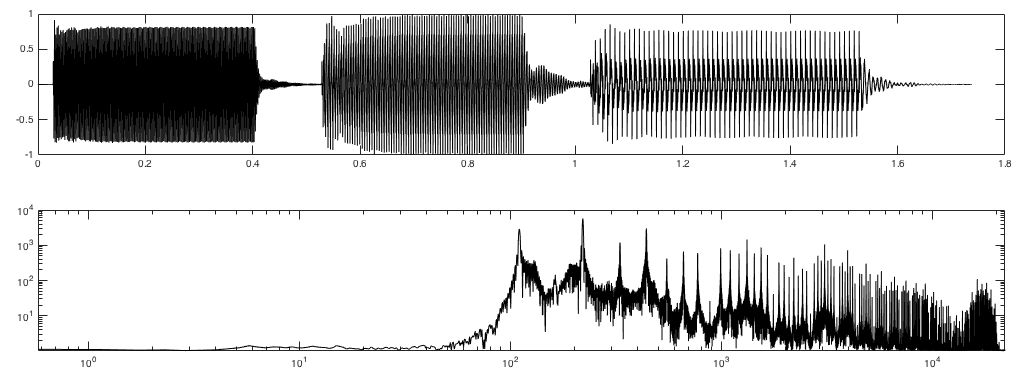
\includegraphics[width=1\textwidth]{bilder/stft01.png}
	\caption[Beispiel für die DFT]{Ein \SI{1.8}{\second} langes Signal. Oben: Der Zeitbereich mit drei klar erkennbaren Tönen. Unten: Das Frequenzspektrum des gesamten Signals mit logarithmierten Achsen.}
	\label{img:stft01}
\end{figure}

Es ist wünschenswert, einen Kompromiss aus den Vorteilen beider Bereiche zu finden, indem man das Spektrum kürzerer Zeitabschnitte des Signals bildet. Hierzu wird der Zeitbereich $x[\;]$ in Fenster der Länge $M$ zerlegt. Die zeitliche Differenz zwischen zwei Fenstern wird als \emph{Hop Size} $R$ bezeichnet. \autoref{eq:signal-Window} definiert die Bildung des \emph{Signalfensters} $x_i[\;]$. Die komplette Zerlegung eines Signals in Signalfenster wird als \emph{Windowing} bezeichnet.\cite{juliusSmith}

\begin{equation}
x_{i}[n] = x[n+i\cdot R]
\label{eq:signal-Window}
\end{equation}

\begin{figure}[h]
	\centering
	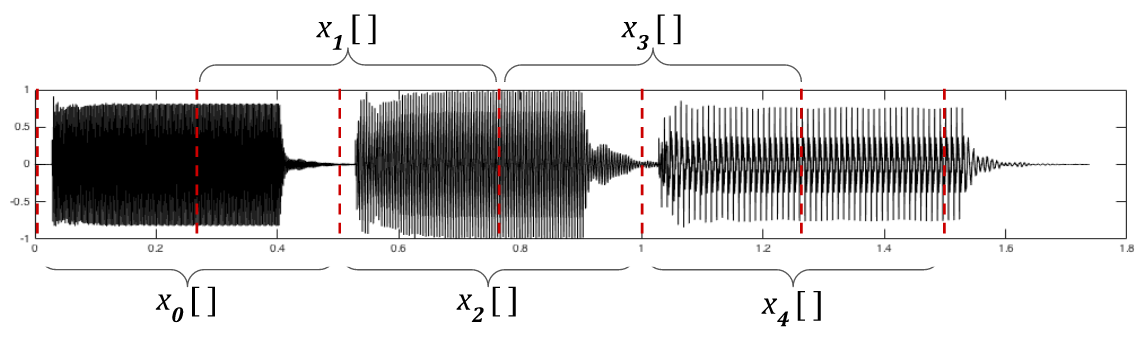
\includegraphics[width=1\textwidth]{bilder/signalWindows02.png}
	\caption{Windowing: Die Zerlegung eines Signals in kürzere Fenster.}
	\label{img:siganlWindows}
\end{figure}

\autoref{img:siganlWindows} zeigt ein Beispiel für die Zerlegung eines Signals $x[\;]$ in die Signalfenster $x_0[\;] ,\ldots, x_4[\;]$. Die Samplingrate des Signals ist $f_s = 44100$, die Fensterlänge beträgt $M = 22050 / f_s = \SI{0.5}{\second}$ und die Hop Size $R = M / 2= \SI{0.25}{\second}$.

Als Vorbereitungsschritt für die Transformation der Signalfenster in den Frequenzbereich wird jedes Signalfenster mit einer \emph{Fensterfunktion} (engl. \emph{window}) $w[\;]$ multipliziert.\cite[S. 69]{sprachverarbeitung} \autoref{eq:hammingWindow} definiert eine der am weitesten verbreiteten Fensterfunktionen, das \emph{Hamming-Window}. Der Paramter $M$ gibt die Länge des Fensters an. \autoref{img:hamming} visualisiert das Hamming-Window.\cite[S. 286]{dspGuide}

\begin{equation}
w[n] = 0.54 - 0.46 \cos(\frac{2\pi n}{M} )
\label{eq:hammingWindow}
\end{equation}

\begin{figure}[h]
	\centering
	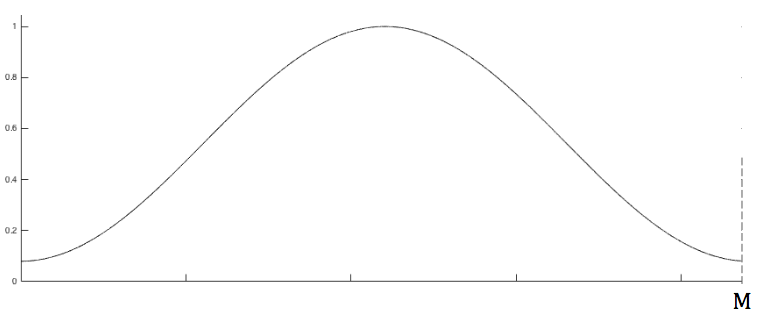
\includegraphics[width=0.5\textwidth]{bilder/hamming01.png}
	\caption{Das Hamming-Window}
	\label{img:hamming}
\end{figure}

\autoref{eq:stft} definiert die \emph{Kurzzeit-Fourier-Transformation} (engl. \emph{Short Time Fourier Transformation}, kurz \emph{STFT}), implementiert mit Hilfe der DFT. Dabei wird das Signalfenster $x_i[\;] = x[n+i\cdot R]$ mit der Fensterfunktion $w[\;]$ multipliziert und in das \emph{Frequenz-Fenster} $X_i[\;]$ transformiert.\cite[S. 69]{sprachverarbeitung} \cite{stft} \autoref{img:stft02} visualisiert die STFT des Beispielsignals aus \autoref{img:siganlWindows}.

\begin{equation}
X_i[k] = \sum_{n=0}^{M-1} x[n+i\cdot R] \cdot w[n] \cdot e^{-j 2\pi k \frac{n}{N}}
\label{eq:stft}
\end{equation}

\begin{figure}[h]
	\centering
	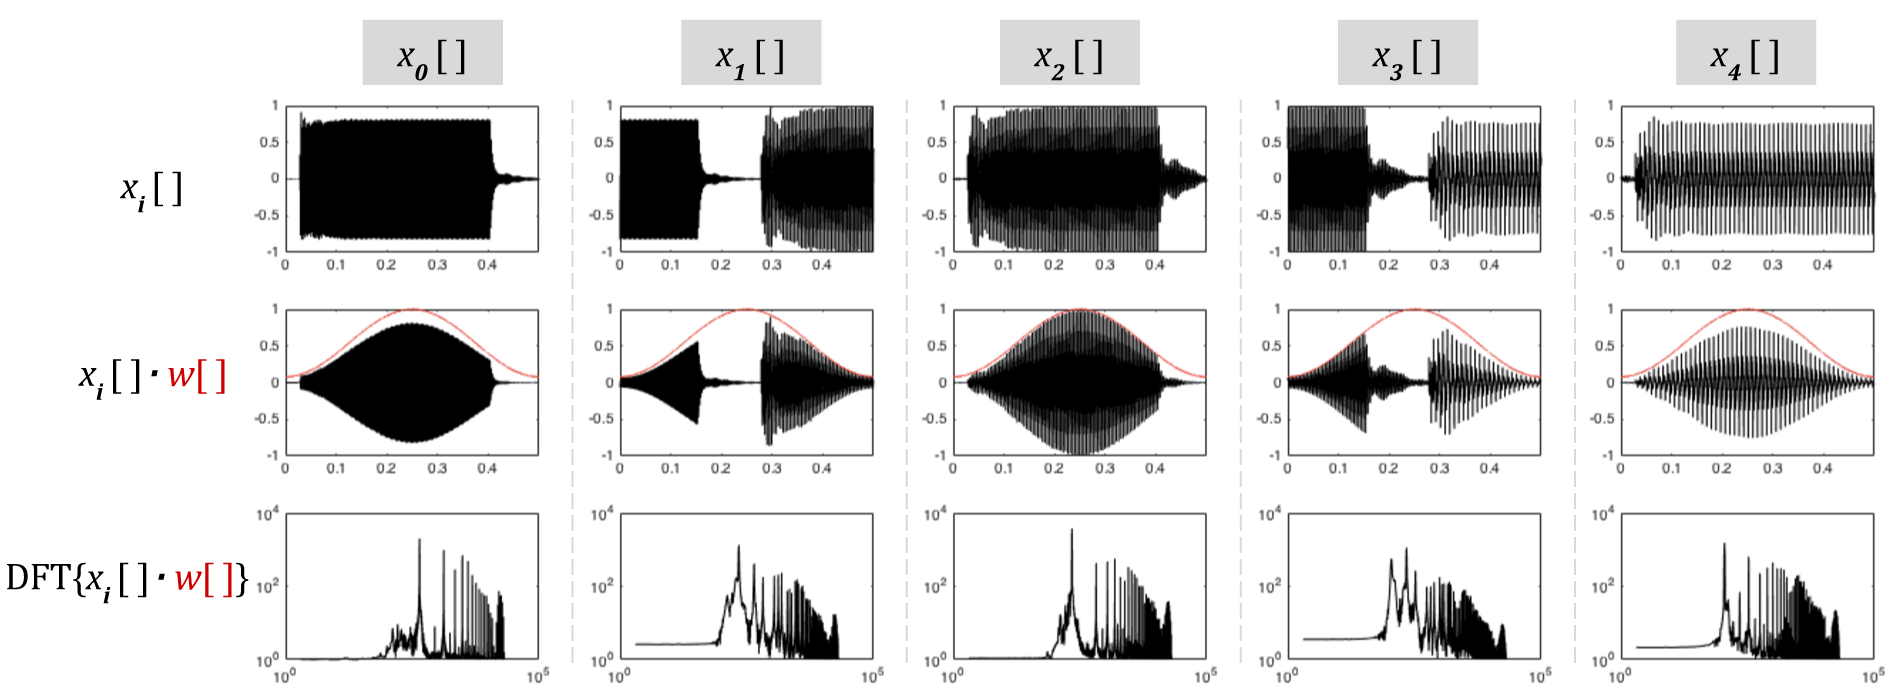
\includegraphics[width=1\textwidth]{bilder/signalWindows03.png}
	\caption{STFT des Beispielsignals aus \autoref{img:siganlWindows}}
	\label{img:stft02}
\end{figure}


\subsection{Akustische Modellierung der menschlichen Stimme}
\label{sec:theVoice}

Der menschliche Sprechapparat wird in die folgenden Komponenten unterteilt:

\begin{description}

\item[Schallproduktion: ] Die Lunge stößt Luft aus, welche die Stimmbänder passiert. Sind die Stimmbänder leicht gespannt, so wird der Luftstrom periodisch unterbrochen. Die Schwingfrequenz beträgt bei erwachsenen Männern etwa \SI{120}{\hertz} und bei Frauen \SI{220}{\hertz}. Die Frequenz kann während des Sprechens um bis zu einer Oktave variieren. So wird ein periodisches Signal produziert, bezeichnet als \emph{Periodische Quelle} (engl. \emph{Periodic Source}). Sind die Stimmbänder stark gespannt, so entstehen Turbulenzen, die sich akustisch als ein zischendes Geräusch ohne identifizierbare Tonhöhe äußern. Dieses stimmlose Signal wird bezeichnet als \emph{Turbulenzquelle} (engl. \emph{Turbulence Source})
\item[Klangformung: ] Das Signal der Stimmlippen passiert den Rachen, Mund- und Nasenraum, welche gemeinsam als \emph {Vokaltrakt} bezeichnet werden. Das Halszäpfchen bestimmt, ob der Luftstrom in den Mund- oder Nasenraum geleitet wird. Die Stellung der Artikulatoren, bestehend aus dem Kiefer, der Zunge usw. bestimmen die Beeinflussung des Klangs des Signals, das durch die Stimmbänder erzeugt wird. Diese Beeinflussung wird als lineares, zeitinvariantes Filter angenähert.\cite[S. 62]{cryModel} \cite[S. 13]{sprachverarbeitung} \autoref{img:schematicVocalOrgans} visualisiert diese Komponenten.
\end{description}

\begin{figure}[h]
	\centering
	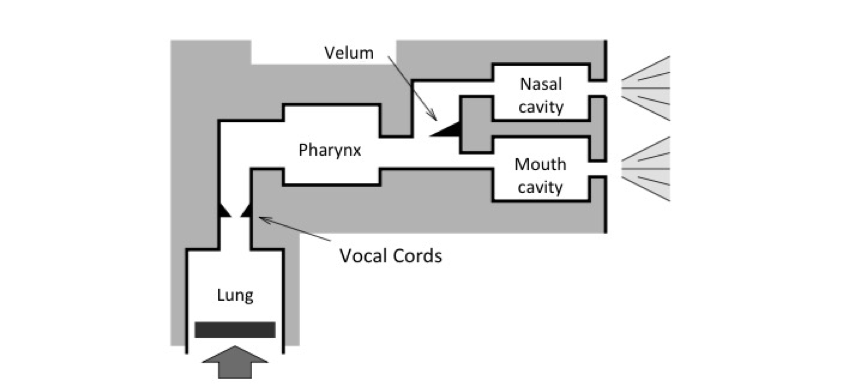
\includegraphics[width=0.7\textwidth]{bilder/SchematicVocalOrgans.png}
	\caption[Schematische Übersicht über die Organe des Sprechapparates]{Schematische Übersicht über die Organe des Sprechapparates. Lung = Lunge, Vocal Chords = Stimmbänder, Pharynx = Rachen, Velum = Halszäpfchen, Mouth Cavity = Mundraum, Nasal Cavity = Nasenraum \cite{speechProduction}}
	\label{img:schematicVocalOrgans}
\end{figure}	

In der Signalverarbeitung wird die menschliche Lautproduktion durch das sogenannte \emph{Source-Filter-Modell} modelliert. Der durch die Stimmbänder erzeugte, periodische Ton wird angenähert durch einen Impuls-Zug, welcher durch den Schlund als lineares Filter moduliert wird. Das stimmlose, nicht-periodische Signal wird durch weißes Rauschen angenähert. Der periodische oder nicht-periodische Ton wird als das Eingangssignal $u[\;]$ bezeichnet. Dieses Signal wird an den Vokaltrakt weitergeben, welcher als lineares, zeitinvariantes Filter mit der Impulsantwort $v[\;]$ modelliert wird. Diese Impulsantwort ist abhängig von der Konfiguration der Organe des Vokaltraktes. Die Lippen werden als zweites lineares, zeitinvariantes Filter mit der Impulsantwort $r[\;]$ modelliert. $r[\;]$ wird auch als \emph{Radiant Model} bezeichnet. Das tatsächliche Sprachsignal $y[\;]$ entsteht somit durch die Faltung des Signals $u[\;]$ mit den beiden linearen, zeitinvarianten Filtern nach \autoref{eq:source-Filter-Model}. \autoref{eq:source-Filter-Model2} definiert den Frequenzbereich des Ausgangssignals $Y[\;]$ durch die Multiplikation der Frequenzbereiche der drei Komponenten.\cite[S. 62 - 63]{cryModel} \cite{speechProduction} \autoref{img:source-filter-model} visualisiert diesen Prozess schematisch.

\begin{equation}
u[\;] * v[\;] * r[\;] = y[\;] 
\label{eq:source-Filter-Model}
\end{equation}

\begin{equation}
U[\;] \cdot V[\;] \cdot R[\;] = Y[\;] 
\label{eq:source-Filter-Model2}
\end{equation}

\begin{figure}[H]
	\centering
	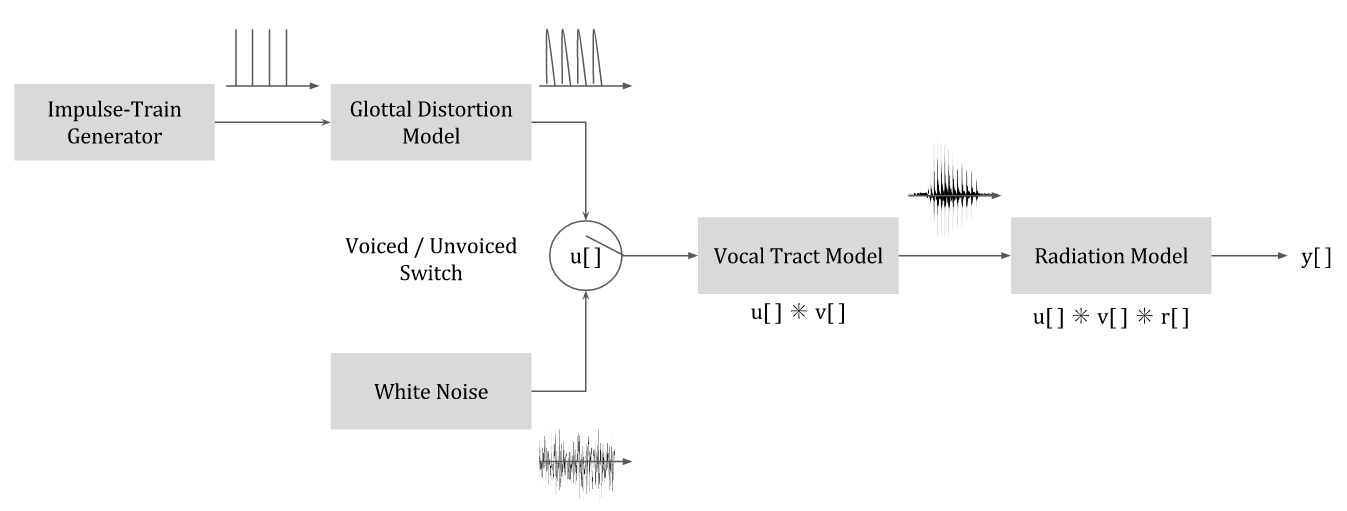
\includegraphics[width=1\textwidth]{bilder/source-filter-model.png}
	\caption[Schematische Übersicht über das Source-Filter-Modell]{Schematische Übersicht über das Source-Filter-Modell (nach: \cite[ \emph{Source estimation}, S. 17]{ricardo_ceps})}
	\label{img:source-filter-model}
\end{figure}	

\autoref{img:glottalSource} zeigt die Zeitbereiche der stimmhaften und der turbulenten Quelle im Vergleich. Wie zu sehen ist, bestimmt der zeitliche Abstand zwischen den Impulsen die Grundfrequenz der Stimme. Dieses Signal $p[\;]$ wird durch den Schlund als Filter $G\{ \; \}$ gefiltert, wodurch der Zeitbereich der periodischen Quelle $G\{p[\;]\} = u_p[\;]$ entsteht. Darunter ist der Zeitbereich des weißen Rauschen zu sehen.\cite[\emph{Source}]{speechAcoustics}

\begin{figure}[h]
	\centering
	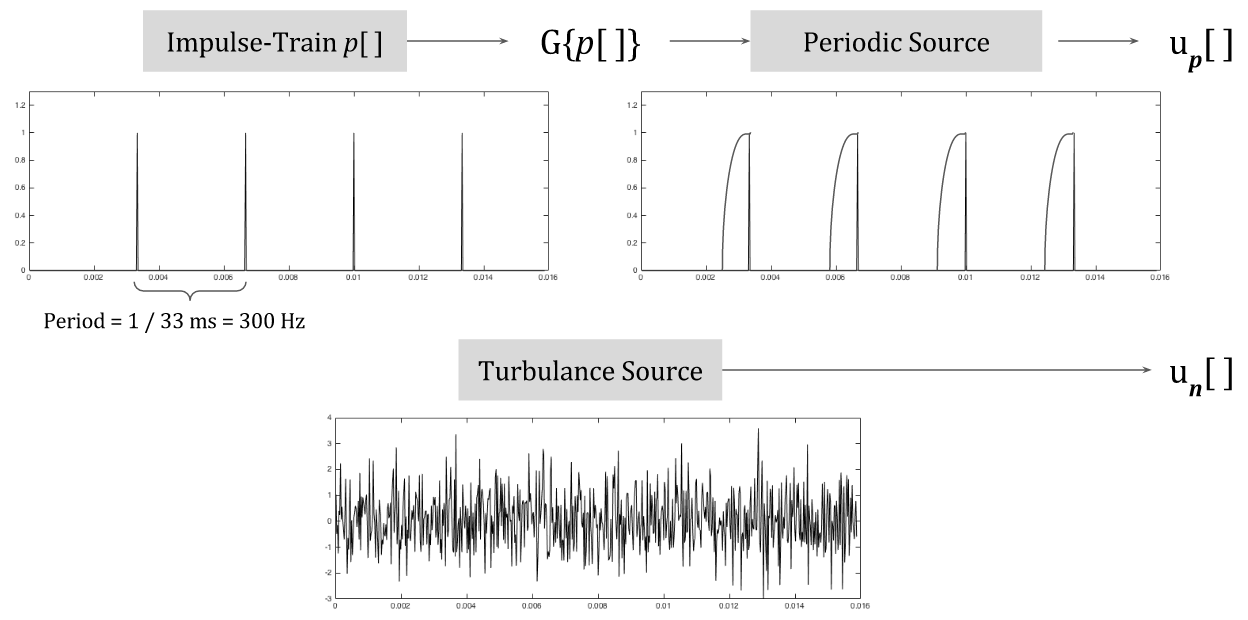
\includegraphics[width=1\textwidth]{bilder/glottalSource.png}
	\caption[Zeitbereiche der periodischen und der turbulenten Quelle]{Zeitbereiche der periodischen und der turbulenten Quelle (nach: \cite[Source]{speechAcoustics})}
	\label{img:glottalSource}
\end{figure}	

\autoref{img:sourceFilerSpectra} zeigt die Frequenzbereiche der Komponenten des Source-Filter-Modells. Die periodische Quelle ($U[\;]$ links) zeichnet sich im Frequenzbereich durch gleichmäßig verteilte Spitzen aus, die mit steigender Frequenz an Amplitude verlieren. Rechts daneben ist der Frequenzbereich des weißen Rauschen zu sehen, welcher einer Zufallsverteilung entspricht. Die Frequenzantwort des Vokaltraktes $V[\;]$ zeichnet sich durch Resonanzfrequenzen aus, von denen in diesem Beispiel vier  erkennbar sind. Die Übertragungsfunktion der Lippen $R[\;]$ wird als Hochpassfilter angenähert. Das Ausgangssignal $Y[\;] = U[\;] \cdot V[\;] \cdot R[\;]$ zeigt den Einfluss der Filter auf das jeweilige Eingangssignal.\cite[\emph{Source estimation}]{ricardo_ceps}, \cite[\emph{Vocal Tract Resonance}]{speechAcoustics}

\begin{figure}[h]
	\centering
	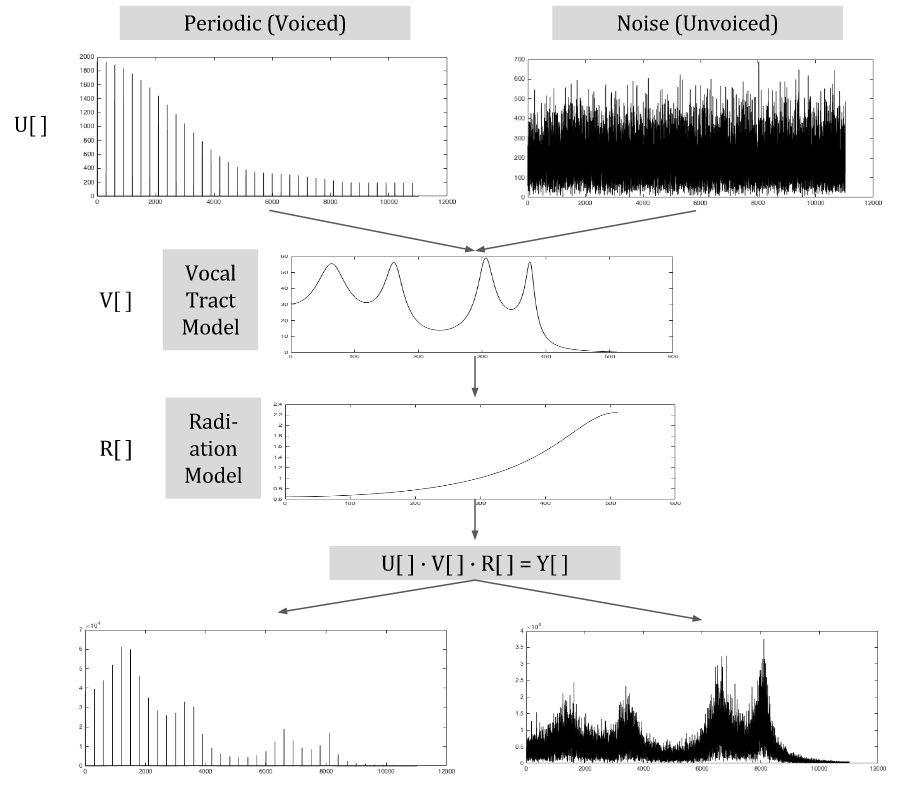
\includegraphics[width=1\textwidth]{bilder/sourceFilterSpectra.png}
	\caption[Betrachtung der Frequenzbereiche des Source-Filter-Modell]{Betrachtung der Frequenzbereiche des Source-Filter-Modell (nach: \cite[\emph{Source Estimation}, S. 3]{ricardo_ceps})}
	\label{img:sourceFilerSpectra}
\end{figure}	

\autoref{img:pitchPeaks} zeigt schematisch das Spektrum eines stimmhaften Sprachsignals. Sowohl die \emph{Grundfrequenz} (engl. \emph{Fundamental Frequency}) als auch die harmonischen Obertonwellen (engl. \emph{Harmonics}) sind rein visuell als \glqq viele, kurze Signalspitzen\grqq{} im Spektrum erkennbar. Der kleinste gemeinsame Teiler der Frequenzen dieser Signalspitzen entspricht der Grundfrequenz $f_0$ des Stimmsignals, in diesem Beispiel $\SI{250.7}{\hertz}$. Die Grundfrequenz ist ebenfalls an der Signalspitze mit der tiefsten Frequenz ablesbar. Die harmonischen Obertöne entsprechen der doppelten, dreifachen,$\ldots\ $ Grundfrequenz, das heißt $2\cdot f_0, 3\cdot f_0, \ldots$ und werden bezeichnet mit $H_1, H_2, \ldots$. Die Grundfrequenz ist \emph{nicht zwingend} die Spitze mit der höchsten Amplitude. Durch den Einfluss des Vokaltraktes als Filter können harmonische Obertöne eine höhere Amplitude als die Grundfrequenz erhalten. Mit Hilfe des Frequenzspektrums lässt sich somit visuell ein stimmhaftes Signal von einem nicht stimmhaften Signal unterscheiden, indem das Spektrum nach dem Vorhandensein regelmäßiger Signalspitzen überprüft wird (vergleiche mit \autoref{img:sourceFilerSpectra}).\cite[S. 52 - 53]{sprachverarbeitung}

% To do: Quelle!!
\begin{figure}[h]
	\centering
	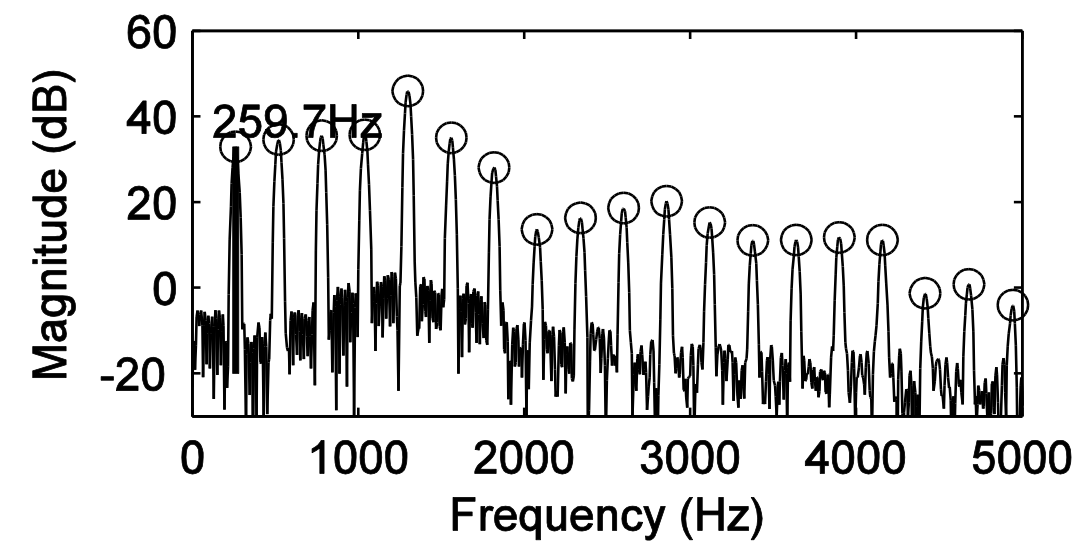
\includegraphics[width=0.5\textwidth]{bilder/pitchPeaks.png}
	\caption[Grundfrequenz und harmonische Obertöne eines stimmhaften Sprachsignals]{Grundfrequenz und harmonische Obertöne eines stimmhaften Sprachsignals \cite{onePitchImage}}
	\label{img:pitchPeaks}
\end{figure}	

\autoref{img:formants} verdeutlicht, wie der als lineares, zeitinvariantes Filter modellierte Vokaltrakt durch Formanten bestimmt wird. Diese Formanten spielen vor allem bei der Beschreibung von Vokalen eine Rolle. Formanten sind lokale Maxima im Spektrum der Transferfunktion, die durch Resonanzen im Vokaltrakt erzeugt werden. Ein Formant wird durch seine Mittenfrequenz, seine Bandbreite und seine Amplitude beschrieben. Die Formanten einer Vokaltraktkonfiguration werden der Reihenfolge ihrer Mittenfrequenzen entsprechend nach dem Schema $F_1 , \ldots , F_n$ nummeriert.  Mit steigender Frequenz nimmt die Amplitude der Formanten ab, der dominanteste Formant ist somit immer der erste. Daher werden meist nur die ersten zwei oder drei Formanten zur Beschreibung eines Vokals angegeben, auch, wenn theoretisch weitaus mehr vom Vokaltrakt erzeugt werden. Für verschiedene Sprachen sind allerlei Tabellen zu finden, welche die Formantenfrequenzen der Vokale auflisten.\cite[S. 19]{sprachverarbeitung}

\begin{figure}[h]
	\centering
	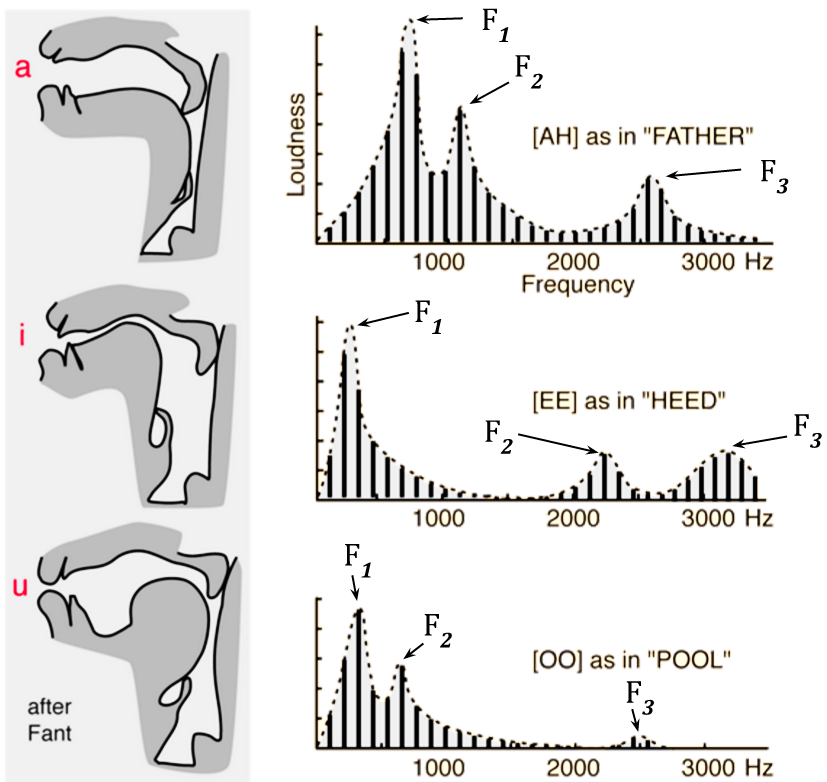
\includegraphics[width=0.65\textwidth]{bilder/formants03.png}
	\caption[Beispiele für Formanten im Sprachsignal]{Beispiele für Formanten im Sprachsignal (nach: \cite{benade})}
	\label{img:formants}
\end{figure}

Beim Sprechen befinden sich sowohl das Signal der Stimmbänder als auch das Filter des Vokaltraktes und der Lippen in ständiger Veränderung. Ein stimmhaftes Sprachsignal gilt nur über kurze Zeitbereiche weniger Millisekunden als periodisch, und selbst in diesen kurzen Zeitbereichen ist die Stimme nicht perfekt, sondern nur annähernd periodisch. Da die Informationen der Sprache vor allem im Frequenzbereich codiert sind, wird die in \autoref{sec:stft} vorgestellte Kurzzeit-Fourier-Transformation zur Analyse von Sprache eingesetzt. Die Visualisierung der Kurzzeit-Fourier-Transformation wird als \emph{Spektogramm} bezeichnet. Dabei werden auf der x-Achse die Zeitpunkte der Fenster und auf der y-Achse die Frequenzen dargestellt. Die Frequenzfenster werden \glqq auf die Seite gelegt\grqq{}, damit der zeitliche Verlauf übersichtlich betrachtet werden kann. Die Amplitude der entsprechenden Frequenzen wird farblich oder durch Helligkeiten codiert, abhängig von der konkreten Implementierung des Spektogramms. Je länger das Zeitfenster der STFT, desto höher ist die Auflösung des Frequenzbereiches und desto niedriger die Auflösung des Zeitbereiches. Je kürzer die Zeitfenster der STFT, desto höher ist die Auflösung des Zeitbereiches, und desto niedriger die Auflösung des Frequenzbereiches.\cite[S. 45 - 50]{sprachverarbeitung} \cite[\emph{Acoustic Representations of Speech}]{speechAcoustics}.

\autoref{img:spectoExample} zeigt ein Beispiel für zwei Spektogramme mit unterschiedlichen Fensterlängen der STFT, angewandt auf einer 9 Sekunden langen Aufnahme eines weinenden Babys. Es ist zu erkennen, dass bei der geringeren Fensterlänge der zeitliche Verlauf besser erkennbar ist, jedoch die einzelnen harmonischen Obertöne weniger gut voneinander unterscheidbar sind. Bei der längeren Fensterlänge sind die Formanten leichter zu unterscheiden, die Anfangs- und Endzeitpunkte der Lautäußerungen sind jedoch schwerer zu lokalisieren.

\begin{figure}[H]
	\centering
	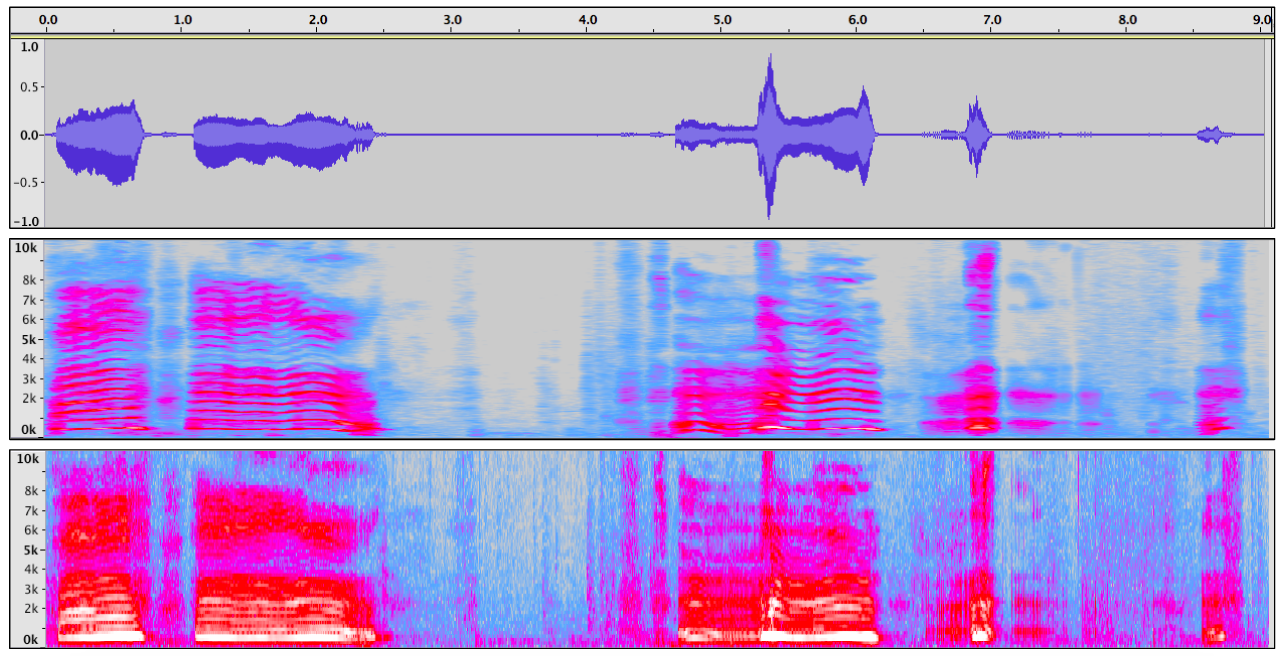
\includegraphics[width=1\textwidth]{bilder/spectogram03.png}
	\caption[Spektogramm einer Audioaufnahme eines Babys]{Oben: Zeitbereich einer Audioaufnahme eines weinenden Babys. Mitte: Spektogramm mit einer Fensterlänge von $\SI{185}{\milli\second}$ (8192-Sample DFT). Unten: Spektogramm mit einer Fensterlänge von $\SI{5}{\milli\second}$ (265-Sample DFT). Rot entspricht hohen Amplituden, Blau entspricht niedrigen Amplituden. (Abbildung erzeugt mit dem Programm \glqq Audacity\grqq)}
	\label{img:spectoExample}
\end{figure}	

\section{Schmerz und Weinen bei Neugeborenen}
\label{sec:medicalFoundations} 

Schmerz wird definiert als ein \glqq unangenehmes Sinnes- oder Gefühlserlebnis, das mit tatsächlicher oder potenzieller Gewebeschädigung einhergeht\grqq{}.\cite[S. 438]{PainAssessment01} In der ersten Hälfte des 20. Jahrhunderts war die vorherrschende Meinung, dass Neugeborene keinen Schmerz empfinden können, wodurch sie beispielsweise nach Operationen häufig keine Schmerzmittel verabreicht bekamen. Der aktuelle Stand der Forschung ist, dass Neugeborene im ähnlichen Maße wie Erwachsene Schmerz empfinden können. Die freien Nervenenden, die in der Lage sind, physische Schäden am Körper festzustellen, sind bei Neugeborenen ebenso wie bei Erwachsenen über den Körper verteilt. Die hormonelle Reaktion ist ebenfalls vergleichbar.\cite[S. 402]{PainAssessment03} \cite[S. 438]{PainAssessment01}

\subsection{Schmerz-Scales als Instrument zur Schmerzbewertung}
\label{sec:painScores}

%besseres wort als Gründe!
Schmerz kann durch diverse Ursachen bei Neugeborenen ausgelöst werden. Diese reichen von physischen Schäden, beispielsweise aufgrund von Komplikationen bei der Geburt oder Gewalteinwirkungen, über Erkrankungen, wie Kopfschmerzen oder Infektionen, bis hin zu therapeutischen Prozeduren, wie Injektionen oder der Desinfektion von Wunden. Das Vorhandensein von Schmerz ist anhand diverser physiologischer, biochemischer, verhaltensbezogener und psychologischer Veränderungen erkennbar.\cite[S. 438]{PainAssessment01} Ein Merkmal, welches das Vorhandensein von Schmerz anzeigt, wird als \emph{Schmerzindikator} bezeichnet. Abbildung \ref{img:painIndicators} zeigt eine Überblick über einige Schmerzindikatoren. Ein Beispiel für einen Schmerzindikator ist der \emph{Gesichtsausdruck} (engl. \emph{Facial Expression}). Schmerzindikatoren werden zu sogenannten \emph{Modalitäten} oder \emph{Dimensionen} gruppiert. Ein Beispiel für eine Schmerz-Dimension ist das \emph{Verhalten} (engl. \emph{Behavioral Indicators}). Der Fokus dieser Arbeit liegt auf dem \emph{Weinen}, welcher zu den verhaltensbezogenen Indikatoren zählt.\cite[S. 69 - 70, 81]{PainAssessment02} \cite[S. 2]{overview}

\begin{figure}[H]
	\centering
	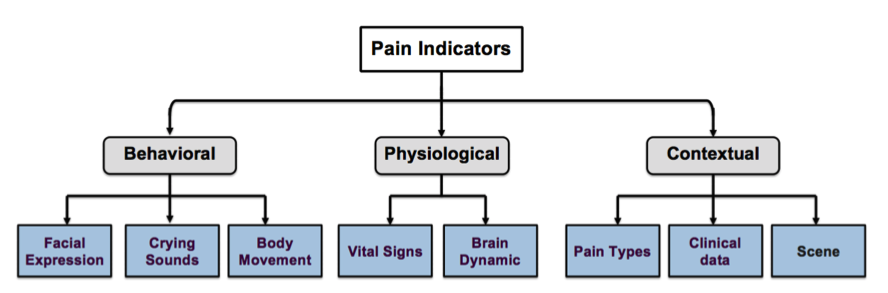
\includegraphics[width=1\textwidth]{bilder/painDimensions.png}
	\caption[Übersicht über Schmerzindikatoren]{Übersicht über eine Auswahl an Schmerzindikatoren \cite[S. 2]{overview}}
	\label{img:painIndicators}
\end{figure}

Schlussendlich ist Schmerz eine subjektive Empfindung. Das heißt, dass ein und der selbe Stimulus bei zwei verschiedenen Personen zu einem unterschiedlichen Schmerzempfinden führen kann. Daher wird der Schmerzgrad bei Erwachsenen typischerweise durch eine Selbsteinschätzung des Patienten unter der Leitung des Arztes festgestellt. Bei Kindern unter drei Jahren ist diese Selbsteinschätzung nicht möglich. Die Schmerzbewertung muss daher von anderen Personen vorgenommen werden. Im klinischen Kontext sind dies medizinische Fachkräfte, wie beispielsweise Ärzte, Krankenpfleger oder Geburtshelfer. Die von außen am leichtesten feststellbaren Indikatoren von Schmerz sind verhaltensbasierte Merkmale. Die Schmerzdiagnostik durch eine andere Person ist, genau wie das Schmerzempfinden, etwas inherent subjektives und abhängig von Faktoren wie dem Alter, Geschlecht, kulturellen Hintergrund, persönlichen Erfahrungen mit Schmerz usw.\cite[S. 1 - 3]{overview} \cite[S. 438]{PainAssessment01} Um die Schmerzdiagnostik objektiver zu gestalten, wurden daher sogenannte \emph{Schmerz-Scales} (engl. \emph{Pain-Scales}) entwickelt, welche mit Hilfe eines Punktesystems den Schmerzgrad des Babys quantifizieren.\cite[S. 240]{painAssessmentStatus} Es existieren \emph{unidimensionale} (auch bezeichnet als \emph{unimodale}) Schmerz-Scales, bei denen der Schmerzgrad aus der Beobachtung \emph{eines} Schmerzindikators geschlossen wird, wie beispielsweise des Gesichtsausdrucks. \emph{Multidimensionale} (auch bezeichnet als \emph{multimodale}) Schmerz-Scales beziehen mehrere Schmerzindikatoren verschiedener Dimensionen in die Schmerzbewertung mit ein. Solche Schmerz-Scales, die mehrere Schmerzindikatoren einer Dimension mit einbeziehen, also beispielsweise nur verhaltensbezogene Schmerzindikatoren, werden je nach Quelle zu den unimodalen oder den multimodalen Schmerz-Scales gezählt. In dieser Arbeit sind mit multimodalen Schmerz-Scales solche gemeint, die prinzipiell mehr als einen Schmerzindikator für die Schmerzbewertung verwenden.\cite[S. 68 - 69, 80 - 81]{PainAssessment02} \cite[S. 1-2, 31]{overview} \cite[S. 404]{PainAssessment03} 

\autoref{tab:nips} zeigt die \glqq Neonatal Infant Pain Scale\grqq{} (NIPS) als Beispiel für eine multimodale Schmerz-Scale. Sie ist für Babys von 0 bis 1 Jahr geeignet und vor allem für die Diagnose von Schmerz gedacht, der während einer Prozedur entsteht. Die Scale wurde auf der Basis der Erfahrungen von Krankenschwestern erarbeitet. Das Baby soll bei der Anwendung dieser Schmerz-Scale für ungefähr eine Minute beobachtet werden. Soll der Schmerz nach einem Eingriff überwacht werden, wird empfohlen, die Diagnose so lange alle 30 Minuten durchzuführen, bis kein Schmerz mehr festgestellt wird. Für jede der aufgeführten Kategorien (Schmerzindikatoren) wird ein \emph{Score} von ein, zwei oder drei Punkte vergeben. Die Scores aller Kategorien werden daraufhin aufaddiert und ergeben den insgesamten \emph{Schmerz-Score} (engl. \emph{Pain-Score}), welcher anschließend interpretiert wird. Bei der NIPS steht ein Schmerz-Score von $>3$ für \glqq moderaten Schmerz\grqq , ein Score von $>4$ für \glqq großen Schmerz\grqq.\cite{nips} \cite[S. 98]{painInNeonates}

\begin{table}[h]

	\centering
	\caption[Neonatal Infant Pain Scale]{Neonatal Infant Pain Scale (NIPS) \cite{nips}}
	\label{tab:nips}
	\begin{tabular}{@{}cccc@{}}
		\toprule
		\textbf{Indicator}     & \textbf{0 points} & \textbf{1 point}     & \textbf{2 points} \\ \midrule
		Facial Expr. & Relaxed           & Contracted           & -                 \\
		Cry               & Absent            & Mumbling             & Vigorous          \\
		Breathing         & Relaxed           & Different than basal & -                 \\
		Arms              & Relaxed           & flexed/stretched     & -                 \\
		Legs              & Relaxed           & flexed/stretched     & -                 \\
		Alertness         & Sleeping          & uncomfortable        & -                 \\ \bottomrule
	\end{tabular}
\end{table}


Es wurden viele weitere multimodale Schmerz-Scales entwickelt, die grundlegend dem Schema der NIPS ähneln. Sie unterscheiden sich hinsichtlich der Schmerzindikatoren, die betrachtet werden, dem Scoring-System, der Art des zu diagnostizierenden Schmerzes, dem Beobachtungszeitraum usw. Einige Schmerz-Scales sind beispielsweise auf die Schmerzdiagnostik während eines Eingriffes spezialisiert, andere auf den darauf folgenden Heilungsprozess. Das Vorgehen zur Schmerzbewertung mit Schmerz-Scales lässt sich folgendermaßen verallgemeinern:

\begin{enumerate}
\item Es wird für jeden Indikator der Schmerz-Scale ein Score nach den angegebenen Kritierien vergeben.
\item Alle Scores werden aufsummiert und ergeben einen insgesamten Schmerz-Score.
\item Der Schmerz-Score wird nach einem von der Schmerz-Scale vorgegebenem Schema interpretiert.\cite{aboutKids}\cite{pat}
\end{enumerate}

In den meisten multimodalen Schmerz-Scales wird das \emph{Weinen} oder \emph{Schreien} (engl. \emph{Cry}) des Babys als Schmerzindikator mit einbezogen.\cite[S. 97 - 98]{painInNeonates} Obwohl Weinen oder Schreien im Deutschen eine negative Konnotation tragen kann, ist in dieser Arbeit mit diesen Begriffen im allgemeinen eine \glqq kindliche Lautäußerung\grqq{} gemeint. 

\autoref{tab:painscores} zeigt eine Übersicht über weitere multimodale Schmerz-Scales. Es sind nur solche Scales enthalten, die das Weinen als Schmerzindikator mit einbeziehen. Für jede Schmerz-Scale wird gezeigt, nach welchen Kriterien das Scoring für das Weinen vorgenommen wird. Ebenfalls werden die weiteren Schmerzindikatoren gelistet, die von der jeweiligen Schmerz-Scale mit einbezogen werden, ohne die Scoring-Systeme für diese Indikatoren detailliert wiederzugeben. Darüber hinaus wird für jede Schmerz-Scale angegeben, für welches Alter und welchen Schmerz-Typ sie vorgesehen ist. Angaben bezüglich der Diagnosehäufigkeit sowie des jeweiligen Beobachtungszeitraums werden gemacht, insofern sie von einer Scale empfohlen wurden. Die Tabelle ist in Englisch verfasst, da alle Quellen der hier gelisteten Schmerz-Scales dem Autor in Englisch vorliegen.

\vspace{-3mm}
\footnotesize
\begin{longtable}{@{}lllll@{}}
	\caption[Übersicht über die Bewertung des Weinens verschiedener multimodaler Schmerz-Scales]{Übersicht über die Bewertung des Weinens verschiedener multimodaler Schmerz-Scales \cite[S. 98 ]{painInNeonates} \cite{flacc} \cite{npass} \cite{bpsn} \cite{cries} \cite{covers} \cite{pat} \cite{dan} \cite{comfort} \cite{bpsn} \cite[S. 71, 75]{PainAssessment02} } \\
\toprule
\textbf{System} & \textbf{S.} & \textbf{Beschreibung des Weinens}                                                                                                                 & \textbf{weitere Indikat.}                                                                                              & \textbf{Sonstiges}                                                                         \\ \midrule
FLACC           & 0           & No cry (awake or asleep)                                                                                                             & \multirow{3}{*}{\begin{tabular}[c]{@{}l@{}}Face, \\ Legs, \\ Activity,\\ Consolability\end{tabular}}             & Age: 2 months - 7 years                                                                   \\
& 1           & \begin{tabular}[c]{@{}l@{}}Moans or whimpers; \\ occasional complaint\end{tabular}                                                   &                                                                                                                  & \begin{tabular}[c]{@{}l@{}}Pain-Type: Ongoing \end{tabular}     \\
& 2           & \begin{tabular}[c]{@{}l@{}}Crying steadily, screams or sobs, \\ frequent complaints\end{tabular}                                     &                                                                                                                  & Observe for: 1 - 5 minutes                                                                        \\ \midrule
N-PASS          & -2          & No cry with painful stimuli                                                                                                           & \multirow{4}{*}{\begin{tabular}[c]{@{}l@{}}Behaviour,\\ Facial Expr.,\\ Extremities,\\ Vital Signs\end{tabular}} & Age: 0 - 100 days                                                                         \\
& -1          & \begin{tabular}[c]{@{}l@{}}Moans or cries minimally \\ with painful stimuli\end{tabular}                                             &                                                                                                                  & \begin{tabular}[c]{@{}l@{}}Pain-Type: Ongoing\\ Observe every: 2 - 4 hours\end{tabular}       \\
& 0           & Appropiate Crying                                                                                                                    &                                                                                                                  &                                                                         \\
& 1           & \begin{tabular}[c]{@{}l@{}}Irritable or Crying at Intervals. \\ Consolable\end{tabular}                                              &                                                                                                                  &                                                                                           \\
& 2           & \begin{tabular}[c]{@{}l@{}}High-pitched or silent-continuous \\ crying. Not consolable\end{tabular}                                  &                                                                                                                  &                                                                                           \\ \midrule
BPSN            & 0           & No Crying                                                                                                                            & \multirow{4}{*}{\begin{tabular}[c]{@{}l@{}}Alertness,\\ Skin Color,\\ Eyebrows,\\ ...\end{tabular}}              & Age: 27 - 41 weeks                                                                                    \\
& 1           & Crying less than 2 minutes                                                                                                           &                                                                                                                  & \begin{tabular}[c]{@{}l@{}}Pain-Type: Procedural\\  \end{tabular}                   \\
& 2           & Crying more than 2 minutes                                                                                                           &                                                                                                                  &                                                                               \\
& 3           & Shrill Crying more than 2 minutes                                                                                                    &                                                                                                                  &                                                                                           \\ \midrule
CRIES           & 0           & \begin{tabular}[c]{@{}l@{}}If no cry or cry which is \\ not high pitched\end{tabular}                                                & \multirow{3}{*}{\begin{tabular}[c]{@{}l@{}}O2,\\ Vital Signs,\\ Expression,\\ Sleeplessness\end{tabular}}        & Age: 0 - 6 Months                                                                         \\
& 1           & \begin{tabular}[c]{@{}l@{}}If cry high pitched but baby. \\ is easily consoled\end{tabular}                                          &                                                                                                                  & \begin{tabular}[c]{@{}l@{}}Pain-Type: Post Operative \\ Observe every: 1 hour\end{tabular}            \\
& 2           & \begin{tabular}[c]{@{}l@{}}If cry is high pitched and \\ baby is inconsolable\end{tabular}                                           &                                                                                                                  &                                                                 \\ \midrule
COVERS        & 0           & No Cry                                                                                                                               & \multirow{3}{*}{\begin{tabular}[c]{@{}l@{}}O2, \\ Vital Signs,\\ Expression,\\ ...\end{tabular}}                 & Age: ?                                                                                    \\
& 1           & High-Pitched or visibly crying                                                                                                       &                                                                                                                  & \begin{tabular}[c]{@{}l@{}}Pain-Type: Procedural \\\end{tabular}                 \\
& 2           & Inconsolable or difficult to soothe                                                                                                  &                                                                                                                  &                                                                     \\ \midrule
PAT            & 0           & No                                                                                                                                   & \multirow{3}{*}{\begin{tabular}[c]{@{}l@{}}Posture,\\ Sleep Pattern,\\ Expression,\\ ...\end{tabular}}           & Age: 0 - 3 months                                                                         \\
& 1           & \multirow{2}{*}{\begin{tabular}[c]{@{}l@{}}When disturbed, doesn’t settle \\ after handling, loud whimper\end{tabular}} &                                                                                                                  & \begin{tabular}[c]{@{}l@{}}Pain-Type: Post Operative\\ Observe every: 1 - 4 h\end{tabular} \\
&             &                                                                                                                                      &                                                                                                                  & Observe for:  15 - 30 sec                                                                 \\ \midrule
DAN           & 0           & Moans Briefly                                                                                                                        & \multirow{3}{*}{\begin{tabular}[c]{@{}l@{}}Facial Exp.,\\ Limb Mov.\end{tabular}}                                & Age: 0 - 2 years                                                                          \\
& 1           & Intermittent Crying                                                                                                                  &                                                                                                                  & Pain-Type: Procedural   \\
& 2           & \begin{tabular}[c]{@{}l@{}}Long-Lasting Crying, \\ Continuous howl\end{tabular}                                                      &                                                                                                                  &                                                                      \\ \midrule
COMFORT        & 0           & No crying                                                                                                                            & \multirow{5}{*}{\begin{tabular}[c]{@{}l@{}}Alertness,\\ Calmness,\\ Respiration,\\ ...\end{tabular}}             & Age: 0 - 3 years                                                                          \\
& 1           & Sobbing or gasping                                                                                                                   &                                                                                                                  & Pain-Type: Post Operative                                                                            \\
& 2           & Moaning                                                                                                                              &                                                                                                                  & Observe every: every Shift                                                                         \\
& 3           & Crying                                                                                                                               &                                                                                                                  &                                                                      \\
& 4           & Screaming                                                                                                                            &                                                                                                                  &                                                                                           \\ \midrule
MBPS            & 0           & Laughing or giggling                                                                                                                 & \multirow{2}{*}{\begin{tabular}[c]{@{}l@{}}Facial Exp.,\\ Movement\end{tabular}}                                 & Age: 2 - 6 Months                                                                                    \\
& 1           & Not Crying                                                                                                                           &                                                                                                                  & \begin{tabular}[c]{@{}l@{}}Pain-Type: Procedural\\ \end{tabular}                 \\
& 2           & \begin{tabular}[c]{@{}l@{}}Moaning quiet vocalizing \\ gentle or whimpering cry\end{tabular}                                         &                                                                                                                  &                                                                      \\
& 3           & Full lunged cry or sobbing                                                                                                           &                                                                                                                  &                                                                                           \\
& 4           & \begin{tabular}[c]{@{}l@{}}Full lunged cry more than \\ baseline cry\end{tabular}                                                    &                                                                                                                  &                                                                                           \\ \bottomrule

	\label{tab:painscores}
\end{longtable}
%\end{table}

\normalsize

Da die Begriffe \emph{Schmerz-Scale} und \emph{Schmerz-Score} in einigen Veröffentlichungen inkonsistent verwendet werden, wird  darauf hingewiesen, dass mit \emph{Schmerz-Scale} das System zur Schmerzdiangostik gemeint ist und mit \emph{Schmerz-Score} die auf Basis der Schmerz-Scale vergebene Punktzahl. Die folgenden Bemerkungen werden weiterhin bezüglich der Schmerz-Scales gemacht:

\begin{itemize}
	
	\item Bei den Schmerz-Scale handelt es sich sowohl bei den Scorings der einzelnen Kategorien als auch bei den Schmerz-Scores um Ordinalskalen. Das bedeutet beispielsweise, dass bei einer Schmerz-Scale ein Schmerz-Score von 4 einen stärkeren Schmerz anzeigt als ein Score von 2, daraus aber nicht geschlossen werden kann, dass der Schmerz doppelt so stark ist. Daraus ergibt sich ebenfalls, dass sowohl die Schmerz-Scores als auch die kategorienbezogenen Scorings verschiedener Schmerz-Scales nicht untereinandet vergleichbar sind. So wird der höchst mögliche Schmerz-Score beispielsweise bei der NIPS mit 7 \cite{nips}, bei der FLACC mit 10 \cite{flacc} und bei der PAT mit 20 \cite{pat} definiert. Ein Schmerz-Score lässt sich folglich nur bei Kenntnis der verwendeten Schmerz-Scale interpretieren.
	\item Ein Teil der aufgelisteten Schmerz-Scales ist für die Schmerzbeurteilung während einer Prozedur gedacht. Die Schmerz-Scales, die zur Bewertung von post-operativen oder andauernden (engl. \emph{ongoing}) Schmerzen geeignet sind, nennen in den jeweiligen Anwendungsvorschriften gewisse Diagnosehäufigkeiten. Beispielsweise empfiehlt die PAT-Scale, die Diagnose nach einer Operation stündlich durchzuführen, bis sich der Gesundheitszustand stabilisiert hat. Anschließend sollte eine Schmerzdiagnose alle 4 Stunden stattfinden.\cite{pat} N-PASS empfiehlt nach Operationen eine Diagnose alle 2 bis 4 Stunden.\cite{flacc} Einige Schmerz-Scales definieren informellere Diagnosefrequenzen, sowie die COMFORT-Scale, welche eine Diagnose vorsieht, wenn \glqq Schmerz vermutet wird\grqq{}, direkt vor und 30 Minuten nach einer Medikation, sowie zu Beginn jedes Schichtwechsels.\cite[S. 241]{painAssessmentStatus}
	
	\item Bei Schmerz-Scales, welche für die Schmerzbeurteilung von Prozeduren gedacht sind, bedingt der Zeitraum der Prozedur den Zeitraum der Schmerzbewertung. Von den Scales, die für andauernde Schmerzen und für die post-operative Begutachtung vorgesehen sind, definieren einige konkret, wie lange das Baby für die Diagnose beobachtet werden soll, um den Schmerz-Score festzulegen. Die PAT empfiehlt eine Beobachtung von 15 bis 30 Sekunden \cite{pat}, FLACC 1 bis 5 Minuten bei wachen und mehr als 5 Minuten bei schlafenden Patienten.\cite{flacc} Schmerz-Scales, die keine festen Beobachtungszeiträume festlegen, implizieren diese durch die Kriterien der Schmerzbewertung. Die FLACC beispielsweise bewertet ein Weinen mit einem Score von 2, wenn es \glqq stetig\grqq{} ist und DAN vergibt einen Score von 2 für \glqq lang anhaltendes Weinen\grqq. \cite{flacc} Die BPSN schließt den Schmerzgrad vor Allem aus der Länge des Weinens.\cite{bpsn} Die nicht explizite Definition der Beobachtungszeiträume stellt eine Schwierigkeit bei Schmerz-Scales dar, da sie die Vergleichbarkeit der Bewertungsergebnisse verschiedener diagnostizierender Personen mindert.\cite[S. 100]{painInNeonates}
	
	\item Die Kriterien zum Scoring des Weinens werden zum größten Teil mit \emph{subjektiv behafteten Begriffen} beschrieben. Beispielsweise wird bei dem \emph{N-PASS}-System ein Score von drei für \glqq High-pitched or silent-continuous crying\grqq{} vergeben. Die Begriffe \glqq high-pitched\grqq{} und \glqq silent-continuous\grqq{} werden nicht näher definiert. Auch die Anwendungsvorschriften der Schmerz-Scales geben keine festen Definitionen. Dies erleichtert den praktischen Einsatz der Scales, führt jedoch zu einem Interpretationsspielraum und somit zu einem von der diagnostizierenden Person abhängigen Scoring. Die \emph{BPSN}-Scale nutzt als einzige der vorgestellten Scales objektiv messbare Eigenschaften in Bezug auf das Weinen.
	
	%\item Die Schmerz-Scales fokussieren unterschiedliche Eigenschaften für das Scoring bezüglich des Weinens. Bei \emph{CRIES} ist die Tonhöhe, bei \emph{BPSN} die Länge und bei \emph{COMFORT} die Art des Weinens ausschlaggebend für die Höhe des vergebenen Scores.
	
\end{itemize}


\subsection{Weinen als Indikator für Schmerz}
\label{sec:foundations_cryingMeta}

Die unterschiedlichen Bewertungskriterien bezüglich des Weinens der in \autoref{tab:painscores} gelisteten Schmerz-Scales werfen die Frage auf, welche Eigenschaften des Weinens eines Babys im allgemeinen am stärksten auf Schmerz hinweisen, und ob es diesbezüglich eine \glqq beste\grqq{} Schmerz-Scale gibt. Dieser Frage unterliegen zwei grundlegendere Fragen:

\begin{enumerate}
	\item Ist es möglich, aus den akustischen Eigenschaften des Weinens den motivierenden Grund für die Lautäußerung abzuleiten?  Klingt ein beispielsweise durch Hunger bedingtes Weinen anders als ein durch Schmerz bedingtes?
	\item Ist es möglich, anhand der akustischen Eigenschaften den \glqq Grad\grqq{} dieses motivierenden Grundes abzuleiten?
\end{enumerate}

Die Annahme, dass es möglich sei, aus den Eigenschaften des Weinens den Grund ableiten zu können, wird als \glqq Cry-Types Hypothesis\grqq{} bezeichnet. Der berühmteste Befürworter dieser Hypothese ist eine skandinavische Forschungsgruppe, auch bezeichnet als \glqq Scandinavian Cry-Group\grqq , die die Idee in dem Buch \glqq Infant Crying: Theoretical and Research Perspectives\grqq \cite{crygroup} publik machte. Die Hypothese besagt, dass die Empfindungen \emph{Hunger, Freude, Schmerz, Geburt} sowie \emph{Sonstiges} klare Unterschiede hinsichtlich der akustischen Merkmale des Weinens aufweisen würden. Diese Unterschiede seien im Spektogramm sichtbar (siehe \autoref{sec:theVoice}). Wenige Jahre Später zeigten Müller et al. \cite{cryisnoise}, dass bei leichter Veränderung der Experimentbedingungen die Unterscheidung nicht mehr möglich sei. Die Gegenhypothese ist, dass Weinen \emph{nichts als undifferenziertes Rauschen} sei.\cite[S. 9 - 13]{signal} Bis heute liegt nach Kenntnis des Autors kein anerkannter Beweis für die eine oder andere Hypothese vor. Es gibt lediglich starke Hinweise dafür, dass sich die Plötzlichkeit des Eintretens des Grundes in den akustischen Eigenschaften des Weinens bemerkbar macht. Ein plötzliches Ereignis, wie ein Nadelstich oder ein lautes Geräusch, führen auch zu einem plötzlich beginnenden Weinen. Ein langsam eintretendes Ereignis, wie ein langsam zunehmender Schmerz oder Hunger führen auch zu einem langsam eintretenden Weinen. Daher wird empfohlen, den Grund für das Weinen aus dem Kontext abzuleiten.\cite[S. 17 - 19]{signal}

Die Zweite Frage nach der Ableitung der Stärke des Unwohlseins aus den akustischen Eigenschaften des Weinens wird unter dem Ausdruck \emph{Cry as a graded Signal} subsumiert. Je \glqq stärker\grqq{} das Weinen, desto höher der Grad des Unwohlsein (\emph{Level of Distress}, kurz \emph{LoD}) des Säuglings. Tatsächlich bemessen wird dabei der vom Beobachter vermutete Grad des Unwohlseins des Babys, und nicht der tatsächliche Grad, da dieser ohne die Möglichkeit der direkten Befragung des Babys nicht mit absoluter Sicherheit bestimmt werden kann. Ein hohes Unwohlsein hat vor allem eine schnelle Reaktion der Aufsichtspersonen zur Beruhigung des Babys zur Folge, womit dem Weinen eine Art Alarmfunktion zukommt. Es gibt starke Hinweise darauf, dass der Level of Distress anhand objektiv messbarer Eigenschaften des Audiosignals bestimmt werden kann. So herrscht beispielsweise weitestgehend Einigung darüber, dass ein \glqq lang\grqq{} anhaltendes Wein auf einen hohen Level of Distress hinweist. Insofern aus dem Kontext des Weinens Schmerz als die wahrscheinlichste Ursache eingegrenzt werden kann, kann aus einem hohen Level of Distress ein hoher Schmerz abgeleitet werden.\cite[S. 13 - 17]{signal}\cite{lod} Es herrscht wiederum keine Einigung darüber, welche akustischen Eigenschaften genau ein hohes Level of Distress anzeigen. Carlo V Bellieni et al. \cite{dan} stellten fest, dass bei sehr starkem Schmerz in Bezug auf die DAN-Scale (siehe \autoref{tab:painscores}) die Tonhöhe steigt. Hingegen weist laut Qiaobing Xie et al. \cite{lod} ein häufiges und dysphoniertes Schreien auf einen hohen Level of Distress hin.

\subsection{Akustische Modellierung und Analyse des Weinens}
\label{sec:acousticModel}

Das Wissenschaftsgebiet, welches sich mit der Analyse und Interpretation des Weinens Neugeborener auseinandersetzt, wird als \glqq Schreiforschung\grqq{} bezeichnet. Die bis heute wohl prominenteste Forschungsgruppe dieses Wissenschaftsgebietes ist die in \autoref{sec:foundations_cryingMeta} erwähnte \glqq Scandinavian Cry-Group\grqq \cite{crygroup}, welche zwischen 1960 und 1990 das Weinen von Babys systematisch erforscht hat. Das wichtigste Werkzeug zur Analyse der Lautäußerungen war das Spektogramm, welches damals auf analogen Technologien basierte. Das Ziel der frühen Schreiforschung war es, mit Hilfe des Spektogramms Muster zur Unterscheidung von einem abnormalem Weinen und einem normalen Weinen zu finden, um beispielsweise Krankheiten erkennen zu können.\cite[S. 142]{signal} 

Teil der Scandinavian Cry-Group waren H. Golub und M. Corwin, die in der Veröffentlichung \glqq A Physioacoustic Model of the Infant Cry\grqq \cite{cryModel} ein Vokabular zur Beschreibung typischer, im Spektogramm erkennbarer Muster festgelegt haben. Da das Vokabular bis heute Einsatz findet, wird an dieser Stelle eine Übersicht über die wichtigsten Begriffe gegeben. Weiterhin werden Begriffe aufgeführt, die von Zeskind et al. in \glqq Rythmic organization of the Sound of Infant Cry\grqq{} verwendet wurden.\cite{rythmic}

Das Weinen von Babys lässt sich im allgemeinen als das \glqq rhythmische Wiederholen eines beim Ausatmen erzeugen Geräusches, einer kurzen Pause, einem Einatmungsgeräusch, einer zweiten Pause, und dem erneuten Beginn des Ausatmungsgeräusches\grqq{} beschreiben.\cite{wolff}

Die folgenden Begriffe werden in \autoref{img:cryVocabulary} veranschaulicht.

\begin{itemize}
	\item \textbf{Expiration (Ausatmung):} Der Klang, der bei einem einzelnen, ununterbrochenen Ausatmen mit Aktivierung der Stimmbänder durch das Baby erzeugt wird. \cite{rythmic}. Der von Golub et al. \cite[S. 61]{cryModel} verwendete Begriff \textbf{Cry-Unit} wird in dieser Arbeit synonym gebraucht und mit \textbf{Schreieinheit} ins Deutsche übersetzt. Umgangssprachlich handelt es sich um einen einzelnen, ununterbrochenen \emph{Schrei}.
	\item \textbf{Inspiration (Einatmung):} Der Klang, der beim Einatmen durch das Baby erzeugt wird.
	\item  \textbf{Burst:} Die Zeit von Beginn einer Ausatmung bis zum Beginn der darauf folgenden Ausatmung. Befindet sich zwischen den beiden Ausatmungen eine Einatmung, so umfasst ein Burst die zeitliche Dauer sowohl der Ausatmung, der Einatmung als auch die beiden Pausen zwischen diesen Geräuschen.\cite{rythmic}
	\item  \textbf{Cry:} Die gesamte klangliche Antwort zu einem spezifischen Stimulus. Eine Gruppe mehrerer Schreieinheiten.\cite[S. 61]{cryModel} In dieser Arbeit wird ein \emph{Cry} auch als \textbf{Cry-Segment} oder \textbf{Schrei-Segment} bezeichnet, um Verwechslungen zu vermeiden.
\end{itemize}

\begin{figure}[H]
	\centering
	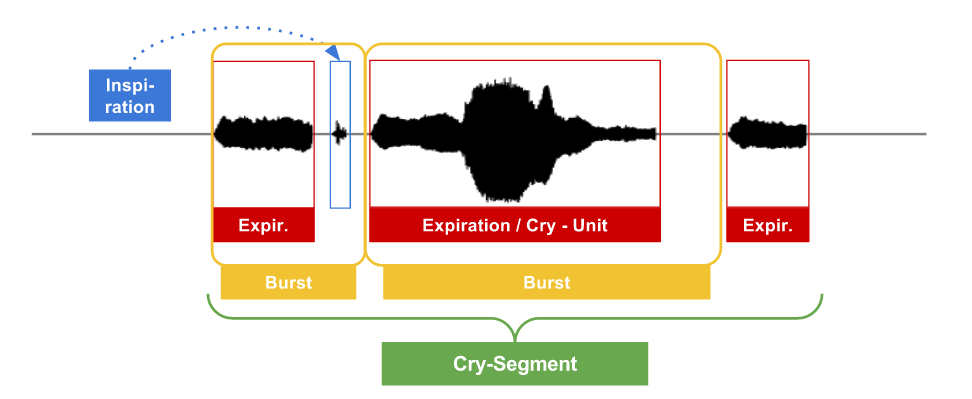
\includegraphics[width=0.9\textwidth]{bilder/cryVoc02.png}
	\caption{Veranschaulichung des Grundvokabulars}
	\label{img:cryVocabulary}
\end{figure}

Schreieinheiten werden von H. Golub und M. Corwin in eine der drei folgenden Kategorien eingeordnet, bezeichnet als \emph{Cry-Types} oder \emph{Cry-Modes}:

\begin{itemize}
	\item \textbf{Phonation} beschreibt eine Schreieinheit mit \glqq voller Vibration der Stimmbänder\grqq{} und einer Grundfrequenz zwischen 250 und \SI{700}{\hertz}. Entspricht umgangssprachlich einem Weinen mit einem \glqq klaren, hörbaren Ton\grqq{}.
	\item \textbf{Hyper-Phonation} beschreibt eine Schreieinheit mit einer \glqq falsetto-artigen Vibration der Stimmbänder\grqq{} und einer Grundfrequenz zwischen 1000 und \SI{2000}{\hertz}. Entspricht umgangssprachlich einem Weinen mit einem \glqq sehr hohen, aber klar hörbaren Ton\grqq{}.
	\item \textbf{Dysphonation} beschreibt eine Cry-Unit ohne klar feststellbare Tonhöhe, produziert durch Turbulenzen an den Stimmbändern. Entspricht umgangssprachlich dem \glqq Brüllen oder Krächzen\grqq{}.\cite[S. 61 - 62]{cryModel}
\end{itemize}

Die folgenden Eigenschaften können für einzelne Schreieinheiten festgestellt werden:

\begin{itemize}
	\item \textbf{Duration:} Die zeitliche Dauer der Schreieinheit.
	\item \textbf{Duration of Inspiration: }Die zeitliche Dauer der Pause zwischen zwei Schreieinheiten.
	\item \textbf{Grundfrequenz:} Die Grundfrequenz der Stimme wurde erläutert in \autoref{sec:theVoice}. Für eine Schreieinheit kann die durchschnittliche, die höchste und die niedrigste Grundfrequenz sowie die Varianz festgestellt werden.
	\item \textbf{Frequenz der Formanten:} Wie bei der Grundfrequenz kann der Durchschnitt, das Maximum, Minimum usw. für eine Schreieinheit berechnet werden.
	\item \textbf{Ratio2: } Verhältnis zwischen den Energien der Frequenzen unterhalb von \SI{2000}{\hertz} zu den Frequenzen oberhalb von \SI{2000}{\hertz}.
	\item \textbf{Cry-Mode Changes:} Häufigkeit des Wechsels des Cry-Modes innerhalb einer Schreieinheit.
	\item \textbf{Amplitude:} Die Lautstärke der Schreieinheit, gemessen in Dezibel.\cite[S. 85]{parentalPerception} \cite[S. 156]{threeCryTypes}
\end{itemize}

H. Golub und M. Corwin stellten weiterhin eine Reihe von Eigenschaften vor, die das zeitliche Verhalten der Grundfrequenz und der harmonischen Obertöne innerhalb einer Schreieinheit beschreiben.\cite[S. 73]{cryModel} Einige dieser Eigenschaften werden in \autoref{img:cryMelodies} in einem schematischen Spektogramm visualisiert.
\begin{itemize}
	\item \textbf{Pitch of Shift:} Grundfrequenz nach einem schnellen Anstieg zu Beginn der Schreieinheit.
	\item \textbf{Glide:} Kurzes, starkes ansteigen der Grundfrequenz.
	\item  \textbf{Glottal Roll:} Dysphonation, die häufig am Ende einer Schreieinheit nach einem Abfall der Grundfrequenz auftritt.
	\item  \textbf{Vibrato:} Mehr als vier starke Schwankungen der Grundfrequenz innerhalb einer Schreieinheit.
	\item  \textbf{Melody-Type } einer Schreieinheit. Meist: fallend, steigend/fallend, steigend, fallend/steigend, flach. 
	\item  \textbf{Continuity:} Verhältnis zwischen stimmhaften und nicht-stimmhaften Bereichen der Cry-Unit.
	\item  \textbf{Double Harmonic Break:} Das Aufkommen einer zweiten Serie von harmonischen Obertönen zwischen den eigentlichen harmonischen Obertönen einer Schreieinheit.
	\item  \textbf{Biphonation:} Das Aufkommen einer zweiten Grundfrequenz mit eigenen harmonischen Obertönen zusätzlich zu der eigentlichen Grundfrequenz.
	\item  \textbf{Noise Concentration:} Starke Energiespitzen zwischen 2000 und \SI{2300}{\hertz}.
	\item  \textbf{Furcation:} Plötzliches Aufteilen der Grundfrequenz und harmonischen Obertöne in mehrere, schwächere Obertöne.
\end{itemize}

\begin{figure}[H]
	\centering
	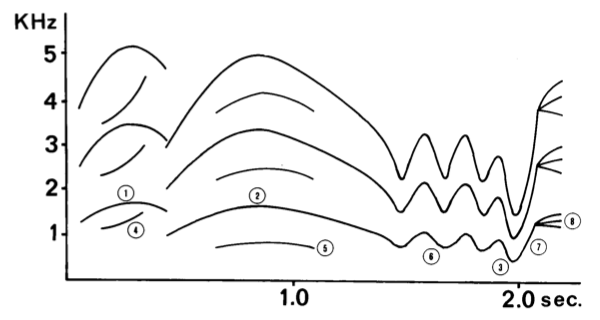
\includegraphics[width=0.7\textwidth]{bilder/melodyTypes.png}
	\caption[Schematisches Spektogramm eines beispielhaften Weinens]{Schematisches Spektogramm eines beispielhaften Weinens zur Visualisierung einiger Eigenschaften. Die schwarzen Linien zeigen  den Verlauf der Grundfrequenz und der Formanten. Die folgenden Eigenschaften werden gezeigt: (1) Pitch of Shift (2) Maximale Grundfrequenz (3) Minimum der Grundfrequenz (4) Biphonation (5) Double Harmonic Break (6) Vibrato (7) Glide (8) Furcation \cite[S. 142]{signal}}
	\label{img:cryMelodies}
\end{figure}

Die folgenden Eigenschaften werden in Bezug auf das gesamte Schrei-Segment, oder zumindest für eine Menge aufeinander folgender Schreieinheiten berechnet:

\begin{itemize}
	\item \textbf{Cry Latence: } Zeit zwischen Stimulus, wie zum Beispiel einem Nadelstich, und der ersten Schreieinheit.
	\item \textbf{Utterances: } Anzahl der Schreieinheiten im Segment.
	\item \textbf{Short Utterances: } Anzahl stimmloser Schreieinheiten im Segment.
	\item ... sowie statistische Auswertungen bezüglich aller in Eigenschaften, die für die Schreieinheiten eines Segmentes definiert wurden, wie beispielsweise der Durchschnitt aller Tonhöhen, Anzahl des Vorkommens bestimmter Melodiekonturen, Varianz der Länge der Schreieinheiten usw.\cite[S. 85]{parentalPerception}
\end{itemize}

Einige Krankheiten wurden in Zusammenhang mit dem vermehrten Vorkommen bestimmter akustischer Eigenschaften des Weinens gebracht. So wurde beispielsweise eine Korrelation zwischen dem Anstieg der durchschnittlichen Grundfrequenz, häufiger Biphonation und geringer Duration und dem Vorhandensein von Gehirnschäden beobachtet. Tendenziell niedrige Grundfrequenzen können auf Trisomie 13, 18 und 21 hinweisen.\cite[S. 85]{parentalPerception}

Ein Problem der Schreiforschung ist, dass sie bis heute weitestgehend unstandartisiert geblieben ist: \cite[S. 142]{signal}
\begin{itemize}
	\item Es gibt keine Liste, welche einen kompletten Überblick über alle (sinnvollen) akustischen Eigenschaften für Schreieinheiten oder Schrei-Segmente gibt. Viele Veröffentlichungen beziehen sich auf die Eigenschaften, die von H. Golub und M. Corwin vorgestellt wurden, und erweitern diese Liste durch eigene Vorschläge. 
	\item Es gibt keine Einigung darüber, welche der Eigenschaften die wichtigsten sind. Beispielsweise haben sich H. Golub und M. Corwin \cite{cryModel} vermehrt auf die Erkennung von Mustern im Melodieverlauf konzentriert, Zeskind et al. \cite{rythmic} haben vermehrt zeitliche Eigenschaften analysiert. Die Eigenschaft, die am häufigsten mit Schmerz, Krankheiten und sonstigen Abnormalitäten in Verbindung gebracht wurde, ist eine abnormal hohe oder niedrige Tonhöhe. Einige Eigenschaften, die von H. Golub und M. Corwin festgestellt wurden, ist nicht einmal gesichert, ob es sich nicht doch um technische Artefakte der damals verwendeten Analogtechnik handelt.\cite[S. 84 - 85]{parentalPerception}
	\item Selbst, wenn in verschiedenen Studien die selben Eigenschaften für das Weinen berechnet wurden, wie zum Beispiel die durchschnittliche Tonhöhe, ist nicht standardisiert, wie dieses zu berechnen ist. Mit \glqq durchschnittliche Tonhöhe des Weinens\grqq{} kann gemeint sein: 1.) die durchschnittliche Tonhöhe, errechnet aus den durchschnittlichen Tonhöhen aller Schreieinheiten. 2.) Die durchschnittliche Tonhöhe aller festgestellten Tonhöhen. 3.) Die durchschnittliche Tonhöhe nur von Ausatmungslauten usw.
	\item Zusammenhänge, die zwischen bestimmten Eigenschaften des Weinens und bestimmten Krankheitsbildern festgestellt wurden, haben häufig eine hohe Spezifität, aber niedrige Sensitivität. So wurde zum Beispiel festgestellt, dass Kinder, die am plötzlichen Kindstot sterben, fast immer eine Erhöhung der Frequenz des ersten Formanten in Verbindung mit häufigen Cry-Mode-Changes zeigen. Viele Babys, die nicht am plötzlichen Kindstot sterben, zeigen jedoch die selben Merkmale.\cite[S. 85]{parentalPerception}
\end{itemize}

\section{Automatisierte Klassifizierung und Bewertung}
\label{sec:learning}

Klassifizierung und Regression sind Teilgebiete des Wissenschaftsgebietes des \emph{Überwachten Lernens}, einem Teilgebiet des \emph{maschinellen Lernens}. Das Ziel beim Überwachten Lernen ist es, ein \emph{Modell}, auch bezeichnet als \emph{Hypothese}, zu entwerfen, welches aus den Eigenschaften einer \emph{Instanz} deren \emph{Kategorie} (auch \emph{Klasse}) oder \emph{Wert} bestimmt. Das Modell wird durch das Generalisieren einer Menge von Beispielen, für die die Klassen oder der Wert bereits bekannt sind, erstellt. Das Modell kann daraufhin eingesetzt werden, um für neue, bisher unbekannte Instanzen die jeweilige Kategorie oder Wert zu prognostizieren.\cite[S. 6 - 7]{machine_marsland}

Diese Begriffe werden anhand eines Beispiels erläutert. Das Ziel ist, für eine Instanz, einem \emph{Baby}, eine Klasse zu prognostizieren, wie zum Beispiel das Geschlecht. Ein Beispiel für einen zu prognostizierenden Wert ist \emph{der Grad des Schmerzes}. Die Prognose wird anhand von zwei Eigenschaften des Babys vorgenommen, und zwar 1.) die durchschnittliche Tonhöhe beim Weinen und 2.) die Augenfarbe. Zur Erstellung des Modells wird eine Datenbank zur Verfügung gestellt, in der für jedes Baby sowohl die Eigenschaften als auch das Geschlecht oder der Schmerzgrad protokolliert wurden.

%Den Feature-kram mit den bezeichnungen nochmal überprüfen!
Die Begriffe werden im folgenden mathematisch konkretisiert: Eine Instanz $x$ ist ein Vektor $x = ( f_1 \in F_1 ,\ \ldots\ , f_n \in F_n )$. $F_i$ wird als \emph{Eigenschaft}, \emph{Feature} oder \emph{Attribut} bezeichnet. In Bezug auf das eben genannte Beispiel ist $F_1 = $ \emph{durschnittliche Tonhöhe} und $F_2 = $ \emph{Augenfarbe}. Ein Beispiel für eine Instanz ist $x = ( \SI{300}{\hertz},$ \emph{blau}). Die Augenfarbe ist ein Beispiel für ein Feature mit einem diskreten Wertebereich, die Tonhöhe ein Beispiel für ein Feature mit einem kontinuierlichen Wertebereich. Die Menge aller möglichen Kombination der Features $F_1 \times , \ldots , \times F_n$ wird als \emph{Feature-Raum} bezeichnet. Der Trainingsdatensatz $D_{trainig}$ besteht aus einer Liste an Instanzen, wobei für jede Instanz die jeweilige Kategorie oder der Wert, gemeinsam Bezeichnet als \emph{Output} oder \emph{Target} $y \in Y$, bekannt ist. Ein Tupel aus einer Instanz und einem Output wird als \emph{Exempel} (engl. \emph{Example}) $e =(x,y)$ bezeichnet. $Y$ bezeichnet die Menge aller möglichen Outputs des Problems. Das heißt, $D_{training} = \big( \; (x_1, y_1), \ldots , (x_N, y_N) \; \big)$. Die Hypothese $H: X \mapsto Y$ ist eine Funktion, die von einer Instanz auf einen Output abbildet. Die Fehlerfunktion $E$ berechnet, wie häufig sich die Hypothese bei der Bestimmung der Targets eines Testdatensatzes $D_{test}$ irrt. Der Test- und der Trainingsdatensatz können die selben Instanzen, teilweise die selben oder gar keine gemeinsamen Instanzen beinhalten.\cite[S. 6 - 7, 18 - 19]{machine_marsland} \cite[S. 8 - 9]{learning_cart_dobra} 

%Nochmal mit den quellen checken!!
Bei der \textbf{Klassifizierung} wird eine Target als \emph{Klasse} bezeichnet. Die Menge aller möglichen Klassen eines bestimmten Problems $Y = \{ y_1 , \ldots, y_n\}$ ist nominal. Das heißt, dass die Menge diskret ist und die Targets einen \emph{qualitativen} Charakter haben. Ein Beispiel für ein Klassifizierungsproblem ist somit die Prognose des Geschlechtes für eine Instanz, also $Y = \{m, w\}$. Die Hypothese wird in diesem Fall als \emph{Klassifikator} $C$ bezeichnet.

Bei der \textbf{Regression} ist die Menge der möglichen Targets eines bestimmten Problems \emph{kontinuierlich} und hat einen \emph{quantitativen} Charakter, womit eine interne Ordnung der Outputs bestimmbar ist. Ein Beispiel für ein Regressions-Problem ist die Prognose des Körpergewichts des Babys mit $Y = \{ \SI{0}{\kilo\gram} , \ldots , \SI{10}{\kilo\gram} \}$. Die Hypothese wird in diesem Fall auch als \emph{Regressor} $R$ bezeichnet.\cite[S. 24]{learning_cart_dobra} \cite[S. 8]{machine_marsland} \cite[S. 28]{statistical_learning}

Handelt es sich bei den Targets um eine Ordinalskala, spricht man von \textbf{Ordinaler Klassifizierung} oder \textbf{Ordinaler Regression}, da die Ansätze zum Lösen solcher Probleme auf den Methoden der Klassifizierung und der Regression aufbauen und miteinander kombinieren.\cite[S. 1]{ordinalClassification} Ein Beispiel für ein solches Problem ist die Prognose des Schmerzgrades, mit $Y = \{ 0 , \ldots, 7  \}$ bei der NIPS (siehe \autoref{tab:nips}).

Es gibt eine Vielzahl an Algorithmen zum Finden des Klassifikators oder Regressors. Welcher Algorithmus der \glqq beste\grqq{} ist, also für einen Testdatensatz eine möglichst hohe \emph{Genauigkeit} oder einen möglichst geringen \emph{Klassifikationsfehler} erzeugt, ist abhängig von der konkreten Problemstellung. Auf die Bestimmung der Genauigkeit wird in \autoref{sec:howGoodIsMyClassifier} eingegangen. Ein Algorithmus, der in dieser Arbeit zur Erkennung der Stimmaktivität in \autoref{sec:vad} eingesetzt wird, ist der \emph{C4.5}-Algorithmus, welcher im folgenden Unterabschnitt erläutert wird.

\subsection{Klassifizierung mit den Algorithmen ID3 und C4.5}
\label{sec:id3}

Der ID3-Algorithmus zählt zu den sogenannten Entscheidungsbäumen, da der durch den Algorithmus entworfene Klassifikator die Form eines Entscheidungsbaumes annimmt. Die Vorraussetzung zur Verwendung des ID-3-Algorithmus ist, dass alle Attribute einen diskreten Wertebereich haben.\cite[S. 54]{machine_mitchell}. \autoref{tab:id3_example} zeigt einen Beispieldatensatz zur Erläuterung des Algorithmus. Die Instanzen sind \emph{Babys}, die Attribute sind $F_1 = $ \emph{Häufigkeit des Weinens} = \{ \emph{oft, normal, selten} \} und $F_2 = $ \emph{Lautstärke des Weinens} = \{ \emph{leise, laut} \}. Die Klasse $Y = $ \{ Ja, Nein \} gibt Auskunft darüber, ob das Baby an chronischen Schmerzen leidet. 

\begin{table}[h]
	\centering
	\caption{Beispieldatensatz für die Kassifizierung mit ID3}
	\label{tab:id3_example}
	\begin{tabular}{cccc}
		\toprule
		$x_i$    & $f_1 \in $ Häufigkeit   & $f_2 \in $ Lautstärke & $y_i \in $ Schmerz \\\midrule
		$x_1$  & oft                & laut          & Ja           \\
		$x_2$  & selten                & laut          & Ja           \\
		$x_3$  & normal                & leise          & Nein         \\
		$x_4$  & selten                & leise          & Nein           \\
		$x_5$  & normal                & laut         & Ja       \\
		$x_6$  & oft                & leise          & Ja       \\ \bottomrule  
	\end{tabular}
\end{table}

\autoref{img:id3tree} zeigt den Klassifikator, den der ID-3 Algorithmus für diesen Datensatz erzeugt. Es handelt sich um einen Entscheidungsbaum. In Jedem Knoten steht ein Attribut, welches einen Ast für jeden möglichen Attributwert bildet. In jedem Blatt steht eine Klasse.\cite[S. 134]{machine_marsland}

\begin{figure}[h]
	\centering
	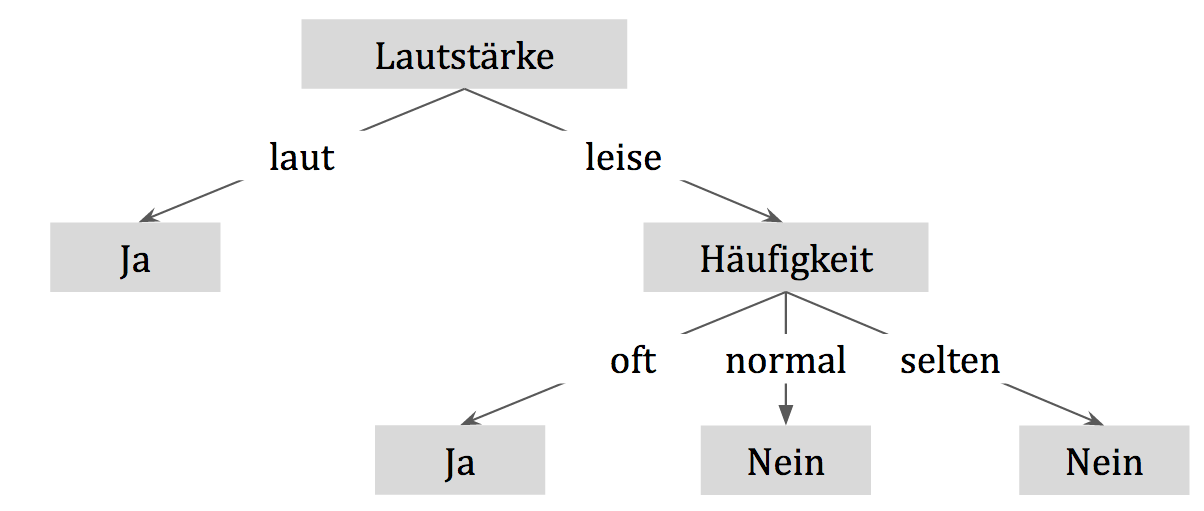
\includegraphics[width=0.65\textwidth]{bilder/id3tree02.png}
	\caption[Beispiel für einen Entscheidungsbaum]{Entscheidungsbaum, der durch den ID3-Algorithmus für den Datensatz aus \autoref{tab:id3_example} erzeugt wird.}
	\label{img:id3tree}
\end{figure}

Der Entscheidungsbaum lässt sich in eine Reihe von \texttt{wenn ... dann ...} -Regeln transformieren. Jeder Weg von der Wurzel bis zu einem Blatt ergibt eine Entscheidungsregel, bei der die Attributwerte der entsprechenden Kanten konjunktiv verknüpft werden und die Klasse implizieren.\cite[S. 134]{machine_marsland} Die Entscheidungsregeln für den Baum aus \autoref{img:id3tree} sind:
\begin{itemize}
	\item \texttt{wenn}  \emph{Lautstärke = laut} \texttt{dann} \emph{Schmerz = Ja}
	\item \texttt{wenn}  \emph{Lautstärke = leise} \texttt{and} \emph{Häufigkeit = oft} \texttt{dann} \emph{Schmerz = Ja}
	\item \ldots
\end{itemize}

Der Entscheidungsbaum wird beim ID3 Algorithmus nach folgendem Muster erstellt: Die Konstruktion wird Top-Down vollzogen, das heißt beginnend bei der Wurzel bis zu den Blättern. In jedem Knoten wird ein Attribut in alle jeweils möglichen Werte aufgespalten. Um an der Wurzel zu entscheiden, welches Attribut zuerst aufgespalten wird, wird jedes Attribut einem statistischen Test unterzogen, um festzustellen, wie \glqq gut\grqq{} es zur Klassifizierung der Trainingsdaten beiträgt. Das \glqq beste\grqq{} Attribut wird ausgewählt und als Wurzel festgelegt. Nun wird ein Ast für jeden möglichen Wert des Attributs gebildet. Der Datensatz des Elternknotens wird in disjunkte Teilmengen aufgeteilt, wobei jedes Kind die Untermenge mit denjenigen Exempeln erhält, die den jeweiligen Attributwert besitzen. Daraufhin beginnt für jedes Kind der Prozess des Auswählens des \glqq besten\grqq{} Attributes von neuem. Ein Kind wird dann zu einem Blatt, wenn seine jeweilige Teilmenge nur noch aus Instanzen einer Klasse besteht und somit kein weiteres Aufteilen notwendig ist.\cite[S. 55]{machine_mitchell}

Zur Quantifizierung der Information wird die Entropie nach \autoref{eq:entropy} als Hilfsmittel definiert. $p_i$ ist die Wahrscheinlichkeit, dass in einem Datensatz $D$ ein Exempel mit der Klasse $i \in Y$ angetroffen wird. Die Entropie quantifiziert die \emph{Unreinheit des Datensatzes}. Ein Datensatz, dessen Exempel alle der selben Klasse angehören, hat die Entropie $0$. Ist die \emph{Unreinheit des Datensatzes} hingegen maximal, das heißt, dass der Datensatz exakt gleich viele Exempel jeder Klasse beinhaltet, ist die Entropie $1$. \cite[S. 135]{machine_marsland}

\begin{equation}
H(p) = -\sum_{i \in Y} p_i \cdot \log_{2} p_i
\label{eq:entropy}
\end{equation}

Es ist das Attribut in einem Knoten zu wählen, welches den höchsten \emph{Informatoinsgewinn} gewährleistet, das heißt, zu einer höchst möglichen \emph{Reinheit} in den Kindsknoten bei der alleinigen Unterteilung des Datensatzes auf Basis dieses Attributs führt. Der Informationsgewinn eines Features $F$ für den Datensatz $D$ wird nach \autoref{eq:informationGain} definiert. $|D|$ ist die Anzahl an Exempeln im Datensatz. $D_f$ ist die Untermenge mit den Exempeln, die für das Feature $F$ den Wert $f$ besitzen.\cite[S. 136 - 137]{machine_marsland}

\begin{equation}
\text{Gain}(D,F) = H(D) - \sum_{f \in F} \frac{|D_f|}{|D|} H(D_f)
\label{eq:informationGain}
\end{equation}

Die Erstellung eines Entscheidungsbaumes mit Hilfe des ID3-Algorithmus wird folgendermaßen als Pseudocode definiert. Der Input des Algorithmus ist der Datensatz $D$ und der Feature-Raum $F_{all}$, der Output ist der Entscheidungsbaum.\cite[S. 139]{machine_marsland}
%% Think about untere Linie entfernen!
\vspace{4mm}

\noindent\textbf{ID3}($D,F_{all}$) \noindent\rule{0.85\linewidth}{0.3pt} \\[-3mm]
\begin{itemize}
\item \textbf{Wenn} alle Examples $e \in D$ das selbe Label haben:
	\begin{itemize}
	\item \textbf{return} eine Blatt mit diesem Label
	\end{itemize}
\item \textbf{Sonst}
	\begin{itemize} 
	\item \textbf{Wenn} keine Attribute übrig sind zum Testen
		\begin{itemize}
		\item \textbf{return} ein Blatt mit dem häufigsten Label in dem Datensatz
		\end{itemize}
	\item \textbf{Sonst:} 
		\begin{itemize}
		\item Wähle das Feature $\hat{F}$ als den nächsten Knoten, dass den Informationsgewinn für den Datensatz $D$ nach \autoref{eq:informationGain} maximiert.
		\item Füge einen Ast für jeden möglichen Wert $f \in \hat{F}$ von dem Knoten hinzu.
		\item Für jeden Ast:
			\begin{itemize}
			\item Berechne $D_f$, in dem $\hat{F}$ von der Liste der Features entfernt wird.
			\item Rufe \textbf{ID3}($D_f, F_{all} / \hat{F}$) rekursiv auf.
			\end{itemize}
		\end{itemize}
	\end{itemize} 
\end{itemize}

\noindent\rule{\linewidth}{0.3pt}

\vspace{3mm}

Der ID3-Algorithmus hat folgende \textbf{Nachteile}:
\begin{itemize}
\item Der Algorithmus akzeptiert keine kontinuierlichen Features.\cite[S. 72]{machine_mitchell}
\item Der Algorithmus neigt zu \emph{Overfitting}. Overfitting bedeutet, dass der Klassfikator $C$ zwar einen möglichst geringen Klassifikationsfehler in Bezug auf den gegebenen Trainingsdatensatz erzeugt, es jedoch einen anderen Klassifikator $C'$ gibt, welcher für diesen speziellen Trainingsdatensatz schlechter performt, jedoch einen geringeren Fehler als $C$ in Bezug auf \emph{alle möglichen Instanzen dieses Problems} erzeugt. Umgangssprachlich formuliert bedeutet Overfitting, dass der Klassifikator den Trainingsdatensatz \glqq auswendig gelernt hat\grqq{} und nicht genügend generalisiert, um auf im Training nicht enthaltene Instanzen angewendet werden zu können. Overfitting im Zusammenhang mit dem ID-3 Algorithmus wird durch \emph{Rauschen im Trainingsdatensatz} bedingt.
\item Der Algorithmus bevorzugt greedy Attribute, die zum Zeitpunkt der Berechnung den höchsten Informationsgewinn gewährleisten. Dabei besteht die Gefahr, dass der Algorithmus in ein lokales Maximum läuft.\cite[S. 66 - 70]{machine_mitchell}
\end{itemize}

Der \emph{C4.5}-Algorithmus erweitert den \emph{ID3}, um dessen Nachteile zu kompensieren. Er ermöglicht die Verwendung kontinuierlicher Attribute und bietet Lösungsansätze zur Verminderung von Overfitting.

Für einen Knoten mit einem kontinuierlichen Attribut werden beim \emph{C4.5}-Algorithmus genau zwei Äste gebildet. Es wird ein Grenzwert für das Feature festgelegt, bei dessen Unterschreitung der linke, und bei dessen Überschreitung der rechte Ast gewählt wird (oder, je nach Implementierung, umgedreht). Das Vorgehen zum Finden eines solchen Grenzwertes ist wie folgt:

\begin{enumerate}
\item Ordne alle Exemple nach ihrem jeweiligen Wert des kontinuierlichen Attributs $F_c$, für das der Grenzwert gesucht wird. 
\item Identifiziere benachbarter Exemple mit unterschiedlichen Klassen. Die Attributwerte dieser Exemple sind mögliche Kandidaten für einen Grenzwert.
\item Berechne den Informationsgewinn bei Setzung des Grenzwertes auf jeden gefundenen Kandidaten. 
\item Wähle denjenigen Grenzwert, der den höchsten Informationsgewinn gewährleistet.\cite[S. 73]{machine_mitchell}
\end{enumerate}

\autoref{img:continuos_variable} visualisiert einen Knoten mit einem kontinuierlichen Attribut $F_c$, der durch einen Grenzwert in zwei Äste aufgespalten wird.


\begin{figure}[h]
	\centering
	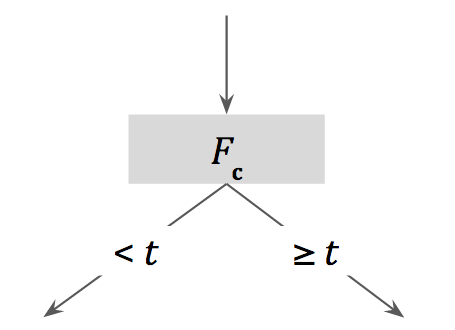
\includegraphics[width=0.3\textwidth]{bilder/continuos_variable.png}
	\caption{Aufspaltung eines kontinuierlichen Attributs im Entscheidungsbaum}
	\label{img:continuos_variable}
\end{figure}


Das als Overfitting beschriebene Problem lässt sich vermeiden, in dem die Tiefe des Entscheidungsbaumes reduziert wird. Diese Begrenzung wird als \emph{Beschneiden} oder \emph{Pruning} bezeichnet. Es gibt grundlegend zwei verschiedene Ansätze:

\begin{description}
 \item[Pre-Pruning:] Ab der Überschreitung einer bestimmten Tiefe wird der Algorithmus frühzeitig gestoppt und ein Knoten, welcher die maximale Tiefe überschreitet, zwangsweise zu einem Blatt umgewandelt. 
 \item[Post-Pruning:] Zuerst wird der komplette Entscheidungsbaum aufgebaut und Overfitting zugelassen. Im Nachhinein wird der Entscheidungsbaum in seiner Tiefe reduziert. Eines der am weitest verbreiteten Post-Pruning-Algorithmen ist das \emph{Reduced Error Pruning}. Dabei wird ein Knoten des Entscheidungsbaumes zu einem Blatt umgewandelt und dem Blatt das Label zugewiesen, welches in seinem Sub-Baum am häufigsten vorkommt. Daraufhin wird der originale Entscheidungsbaum sowie der beschnittene Entscheidungsbaum verwendet, um den Testdatensatz zu klassifizieren. Ist der Klassifizierungsfehler des beschnittenen Baumes nicht höher als der des originalen Baumes, wird das Pruning übernommen. Dieses Vorgehen wird für jeden Knoten des Entscheidungsbaumes angewandt. \cite[S. 68 - 70]{machine_mitchell} 
\end{description}


\subsection{Gütemaße binärer Klassifikatoren}
\label{sec:howGoodIsMyClassifier}

eine binäre Klassifikation ist eine, bei der es genau zwei Klassen gibt, das heißt $|Y| = 2$. Applikationsabhängig werden die beiden Klassen beispielsweise als \emph{Positive} und \emph{Negative}, $1$ und $0$ oder \emph{True} und \emph{False} bezeichnet. Wird bei einer Klassifizierung ein tatsächliches Positive korrekt als Positive prognostiziert, spricht man von einem \emph{True Positive} [TP]. Wird hingegen ein tatsächliches Positive fälschlicherweise als Negative prognostiziert, spricht man von einem \emph{False Negative} [FN]. Bei der Klassifizierung von Negatives spricht man dementsprechend von \emph{True Negatives} [TN] und \emph{False Positives} [FP]. Die \emph{Confusion Matrix} in \autoref{img:Confusion-Matrix} gibt eine Übersicht über die vier möglichen Klassifizierungsergebnisse. \cite[S. 213 - 214]{machine_kubat}

\begin{figure}[h]
	\centering
	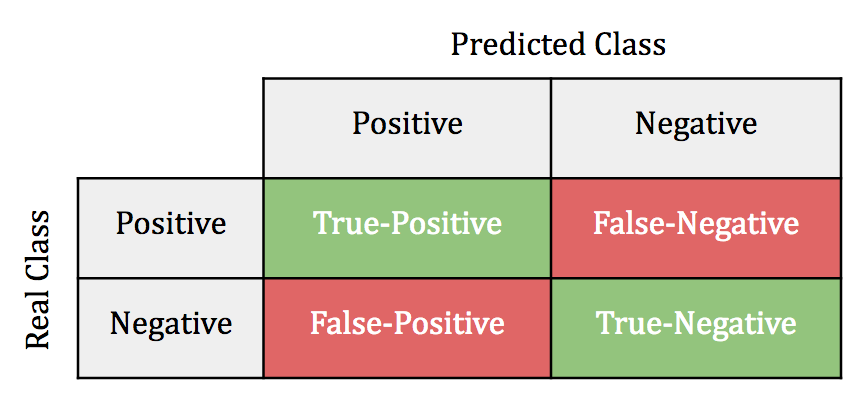
\includegraphics[width=0.6\textwidth]{bilder/Confusion-Matrix02.png}
	\caption[Confusion Matrix]{Confusion Matrix (nach: \cite[S. 214]{machine_kubat})}
	\label{img:Confusion-Matrix}
\end{figure}

Die insgesamte Güte einer Klassifizierung wird durch die \emph{Genauigkeit} (engl. \emph{Accuracy}) nach \autoref{eq:accuracy} bestimmt. Eine Genauigkeit von 100\% bedeutet, dass \emph{alle} Instanzen richtig klassifiziert wurden, eine Genauigkeit von 50\% bedeutet, dass die Hälfte aller Instanzen richtig klassifiziert wurden. Je höher die Genauigkeit, desto geringer der Klassifikationsfehler. \cite[S. 214]{machine_kubat}

\begin{equation}
\text{Accuracy} = \frac{TP+TN}{TP+TN+FN+FP}
\label{eq:accuracy}
\end{equation}

Mit Hilfe der Genauigkeit wird die insgesamte Performance des Klassifikators gemessen. Der Wert allein gibt jedoch keinen Aufschluss darüber, ob der Klassifikator eher eine Tendenz zur falschen Klassifizierung von Positives oder Negatives hat. Bei einer Datenbank mit der selben Anzahl an Positives und Negatives kann eine Genauigkeit von 50\% beispielsweise dadurch entstehen, dass \emph{alle} Instanzen als Positives markiert werden. Das heißt, dass alle Positives richtigerweise als Positives, aber alle Negatives fälschlicherweise ebenfalls als Positives klassifiziert werden. Im umgedrehten Fall ergibt die Klassifizierung aller Instanzen als Negatives ebenfalls eine Genauigkeit von 50\%. In einem dritten Fall irrt sich die Klassifikator gleich oft bei der Einordnung der Negatives und Positives. 

Die Maße \emph{Sensitivität} (engl. \emph{Sensitivity}) und  \emph{Spezifität} (engl. \emph{Specificity}) geben Aufschluss über die Performance des Klassifikators bei der Prognose der Positives und Negatives. Die Sensitivität, auch bezeichnet als \emph{True-Positive-Rate}, bemisst den Anteil tatsächlicher Positives, die auch als solche erkannt wurden, nach \autoref{eq:sensitivity}. Eine Sensitivität von 100\% bedeutet, dass alle in der Datenbasis enthaltenen tatsächlichen Positives auch als solche erkannt  wurden. Die Erkennungsrate der Negatives hat keinen Einfluss auf die Sensitivität. Eine hohe Sensitivität lässt sich somit \glqq einfach\grqq{} erzielen, in dem man \emph{alle} Instanzen immer als Positives klassifiziert.\cite[S. 222]{machine_kubat}

\begin{equation}
\text{Sensitivity} = \frac{TP}{TP+FN}
\label{eq:sensitivity}
\end{equation}

Die Spezifität nach \autoref{eq:specificity} bestimmt analog zur Sensitivität den Anteil der Negatives, die als solche klassifiziert wurden. 

\begin{equation}
\text{Specificity} = \frac{TN}{TN+FP}
\label{eq:specificity}
\end{equation}

Ein Klassifikator, der alle Instanzen als Positives markiert, hat zwar eine Sensitivität von 100\%, aber eine Spezifität von 0\%. Ergeben zwei verschiedene Klassifikationsmodelle sehr ähnliche Genauigkeiten, hilft die Bestimmung der Sensitivität und der Spezifität bei der Auswahl des für den Anwendungsfall adäquateren Klassifikators. So ist beispielsweise bei der Bestimmung von schweren Krankheiten eventuell ein Klassifikator mit höherer Sensitivtät wünschenswert, um die Wahrscheinlichkeit zu minimieren, dass die entsprechende Krankheit nicht erkannt wird.\cite{sens-and_spec}  \cite[S. 222]{machine_kubat}

